% -*- mode: noweb; noweb-default-code-mode: R-mode; -*-
\documentclass[a4paper]{article}

\title{BIP-Predictor}
\author{Marc Wildi\\
Zurich University of Applied Sciences (ZHAW)\\
8000 Zurich, Switzerland\\
marc.wildi@zhaw.ch}



\usepackage{a4wide}
\usepackage{amsmath}
\usepackage{amsfonts} 
\usepackage{amsthm}
\usepackage{ amssymb }
\usepackage[utf8]{inputenc}
\usepackage{hyperref}
\usepackage{float}
\newtheorem{Proposition}{Proposition}
\newtheorem{Corollary}{Corollary}
\newtheorem{Theorem}{Theorem}
\DeclareMathOperator{\sign}{sign}
%- Makes the section title start with Appendix in the appendix environment
\newcommand{\Appendix}
{%\appendix
\def\thesection{Appendix~\Alph{section}}
%\def\thesubsection{\Alph{section}.\arabic{subsection}}
\def\thesubsection{A.\arabic{subsection}}
}

\usepackage{Sweave}
\begin{document}

\maketitle

\begin{abstract}
\noindent 

\end{abstract}

~\\
~\\




%\tableofcontents

\section{Introduction}



\section{Data and Dependence}




\subsection{Data}

\begin{itemize}
\item Choice of indicators: BIP, ip, ESI, ifo, spread
\item Quarterly frequency (emphasize $h\geq 2$)
\item Data transformations: Diff-log, standardization (merely for ease of visual inspection), trim Covid ourliers
\item Revisions and publication lags:  BIP lagged by quarter and ip lagged by two months in Jan-2025 data set
\item Real-time data: all series are artificially aligned at end point. BIP and ip are advanced by their lags.
\end{itemize}

% latex table generated in R 4.2.2 by xtable 1.8-4 package
% Fri May 23 08:04:52 2025
\begin{table}[ht]
\centering
\begin{tabular}{rrrrrr}
  \hline
 & GDP & ip & ifo\_c & ESI & spr\_10y\_3m \\ 
  \hline
2024-07-01 & 902.571 & 90.700 & 85.800 & 92.500 & -1.300 \\ 
  2024-08-01 &  & 93.200 & 84.900 & 90.900 & -1.400 \\ 
  2024-09-01 &  & 91.200 & 83.700 & 89.800 & -1.400 \\ 
  2024-10-01 & 900.761 & 90.800 & 84.100 & 90.700 & -1.200 \\ 
  2024-11-01 &  & 92.200 & 83.800 & 89.300 & -0.900 \\ 
  2024-12-01 &  &  & 82.800 & 86.900 & -0.800 \\ 
  2025-01-01 &  &  & 82.500 & 88.100 & -0.200 \\ 
   \hline
\end{tabular}
\caption{Ragged end.  } 
\label{f_stat}
\end{table}% latex table generated in R 4.2.2 by xtable 1.8-4 package
% Fri May 23 08:04:52 2025
\begin{table}[ht]
\centering
\begin{tabular}{rrrrrr}
  \hline
 & GDP & ip & ifo\_c & ESI & spr\_10y\_3m \\ 
  \hline
2024-05-01 &  & 93.400 & 84.900 & 90.900 & -1.400 \\ 
  2024-06-01 &  & 90.700 & 83.700 & 89.800 & -1.400 \\ 
  2024-07-01 & 902.571 & 93.200 & 84.100 & 90.700 & -1.200 \\ 
  2024-08-01 &  & 91.200 & 83.800 & 89.300 & -0.900 \\ 
  2024-09-01 &  & 90.800 & 82.800 & 86.900 & -0.800 \\ 
  2024-10-01 & 900.761 & 92.200 & 82.500 & 88.100 & -0.200 \\ 
   \hline
\end{tabular}
\caption{Data aligned at sample end.} 
\label{f_stat}
\end{table}

The transformed quarterly series are displayed in Fig. \ref{data}, while Fig. \ref{data_lags} offers a close-up view of the financial crisis and the pandemic. The latter figure illustrates that the real-time GDP and industrial production series are synchronized at dips and peaks (coincident), whereas the other indicators tend to lead in relative terms. This characteristic of the additional explanatory variables can be leveraged in a multivariate approach to enhance forecasting performance compared to univariate benchmarks. 


\begin{figure}[H]\begin{center}\includegraphics[height=3in, width=4.5in]{./Figures/Data.pdf}\caption{Data: standardized log-differences. Data trimmed to $\pm 3$ for ease of visual inspection.\label{data}}\end{center}\end{figure}
\begin{figure}[H]\begin{center}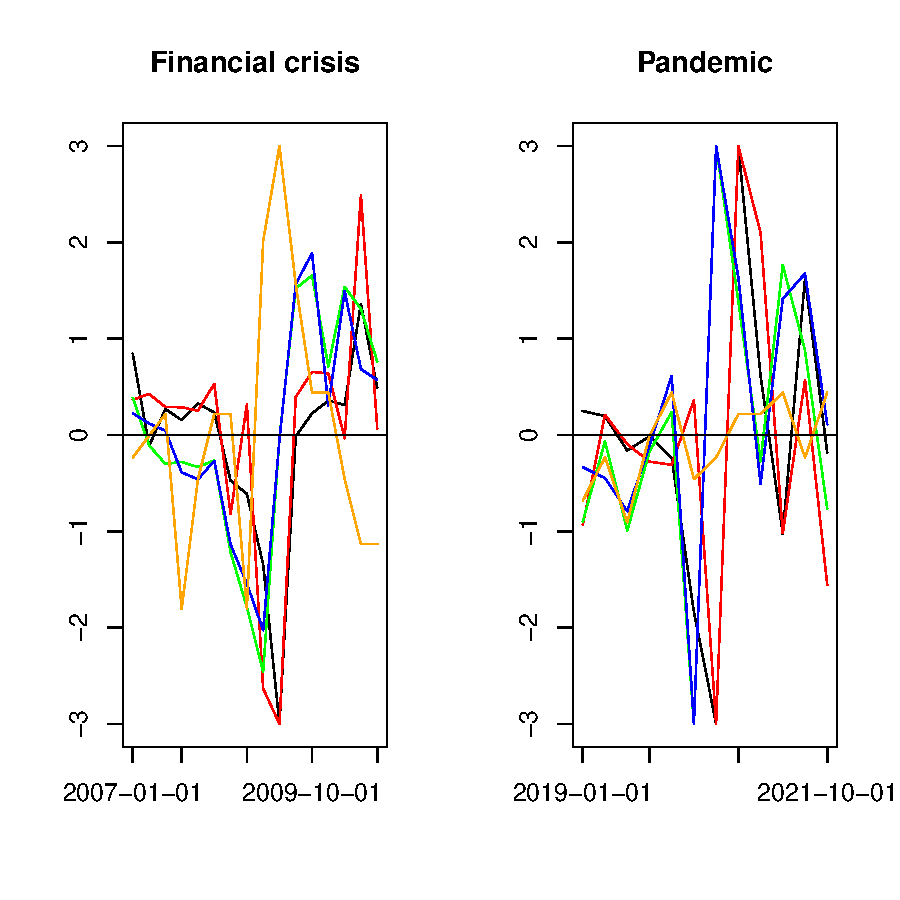
\includegraphics[height=3in, width=4.5in]{./Figures/data_lags.pdf}\caption{Data: leads and lags during financial crisis (left) and Pandemic (right). Data trimmed to $\pm 3$ for ease of visual inspection.\label{data_lags}}\end{center}\end{figure}




\subsection{Dependence}

We analyze the dependence structure of the data and derive a simple VAR model to establish the multivariate filter. The sample cross-correlation function (CCF) is shown in Figs. \ref{CCF} (entire dataset) and \ref{CCF_wc} (data prior to the pandemic).  
\begin{figure}[H]\begin{center}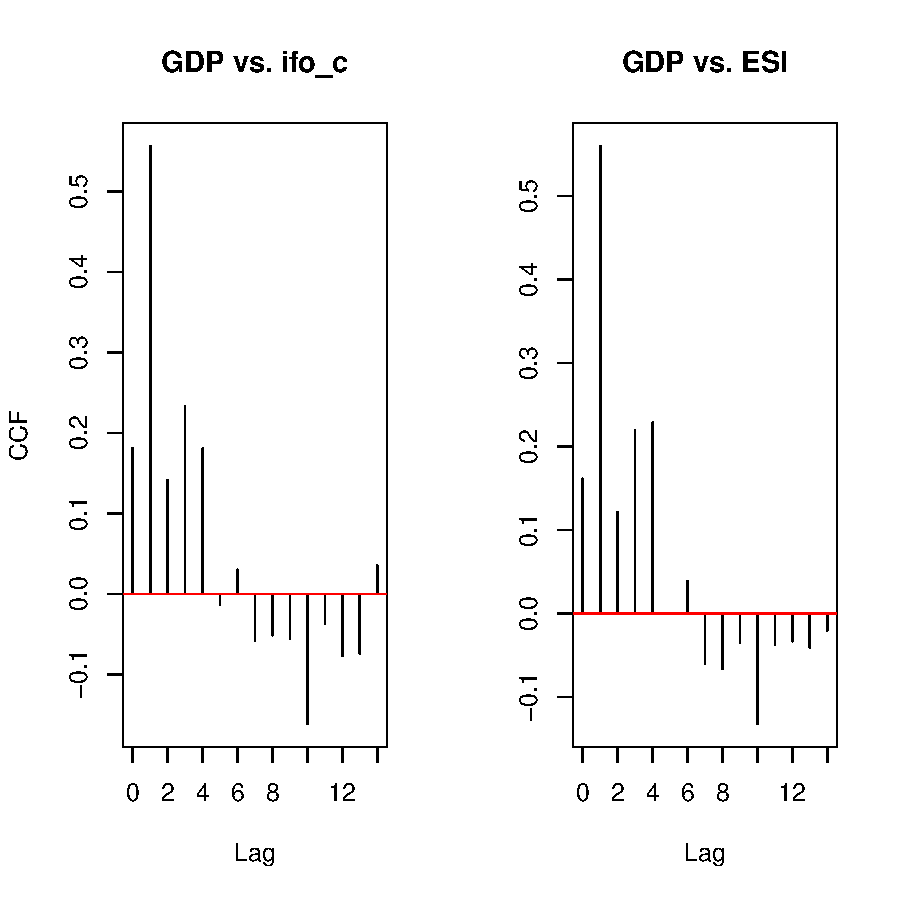
\includegraphics[height=3in, width=4.5in]{./Figures/CCF.pdf}\caption{Sample cross-correlation function: GDP and ifo (left), GDP and ESI (right): full data set, including the pandemic. Correlations at positive lags signify that (real-time) GDP is lagging when referenced against the two (real-time) indicators.\label{CCF}}\end{center}\end{figure}\begin{figure}[H]\begin{center}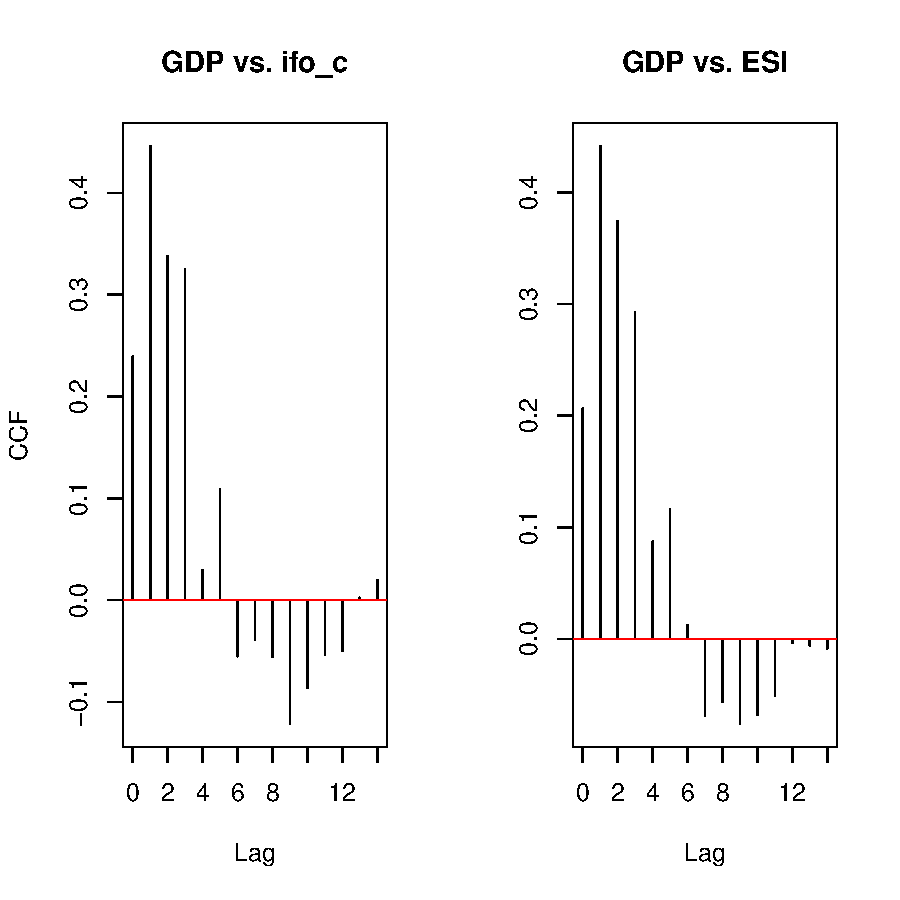
\includegraphics[height=3in, width=4.5in]{./Figures/CCF_wc.pdf}\caption{Sample cross-correlation function: GDP and ifo (left), GDP and ESI (right): without pandemic. Correlations at positive lags signify that (real-time) GDP is lagging when referenced against the two (real-time) indicators.\label{CCF_wc}}\end{center}\end{figure}The CCF confirms the leads and lags illustrated in Fig. \ref{data_lags}, although the strength of the dependence is influenced by the singular readings during the pandemic\footnote{We discard the corresponding data when finalizing the predictor.}. We can now fit a VARMA model, and according to standard diagnostic tests (not shown here), a simple VAR(1) specification aligns with the data. The resulting impulse responses of the model are presented in Figs. \ref{impulse} (full data set) and \eqref{impulse_wc} (prior the pandemic).
\begin{figure}[H]\begin{center}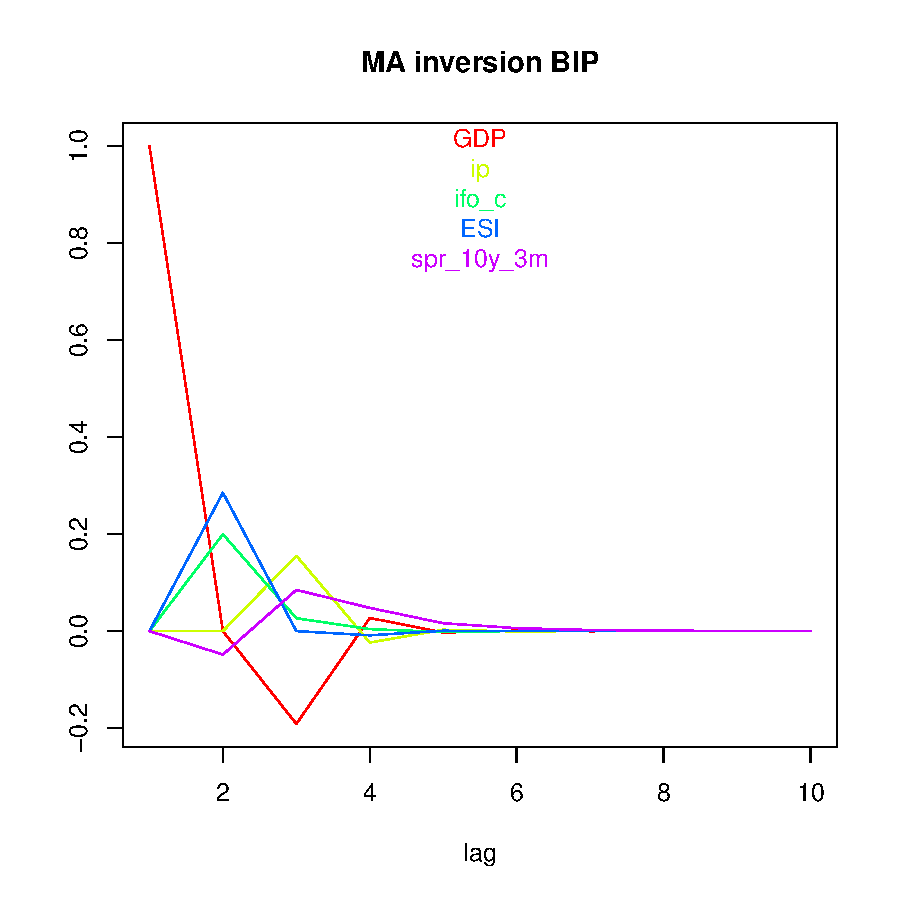
\includegraphics[height=3in, width=4.5in]{./Figures/ma_inv_multi_ip.pdf}\caption{MA inversion of VAR(1): full data set.\label{impulse}}\end{center}\end{figure}\begin{figure}[H]\begin{center}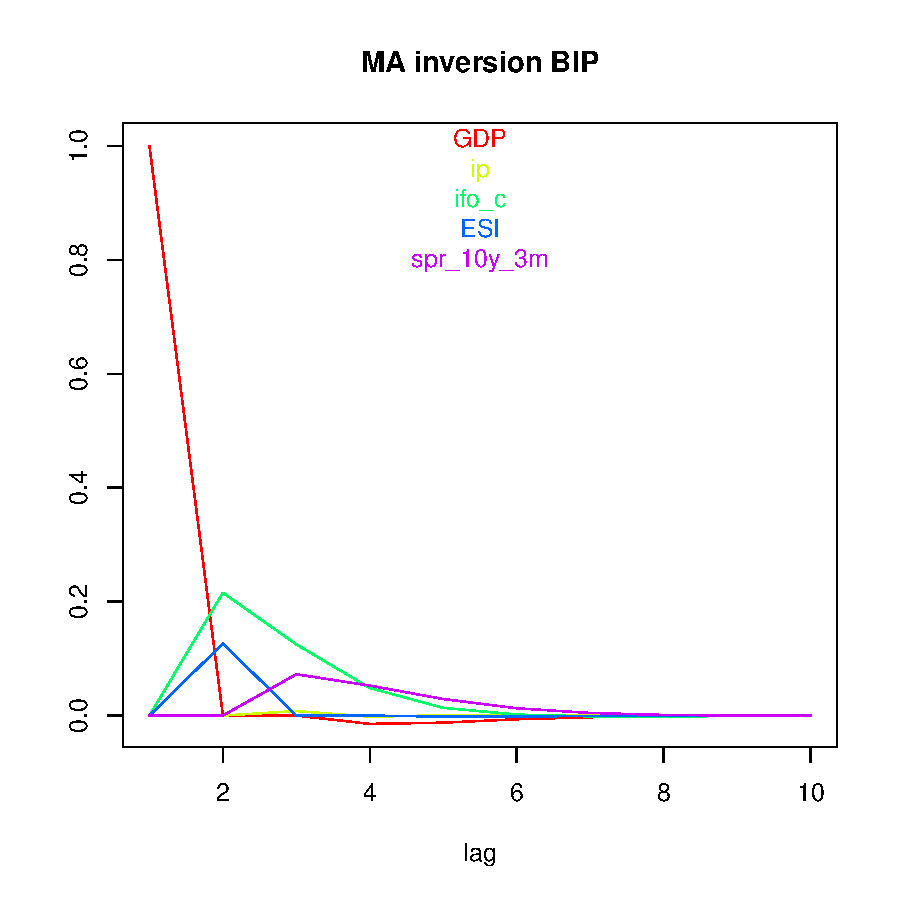
\includegraphics[height=3in, width=4.5in]{./Figures/ma_inv_multi_ip_wc.pdf}\caption{MA inversion of VAR(1): without Pandemic.\label{impulse_wc}}\end{center}\end{figure}\begin{figure}[H]\begin{center}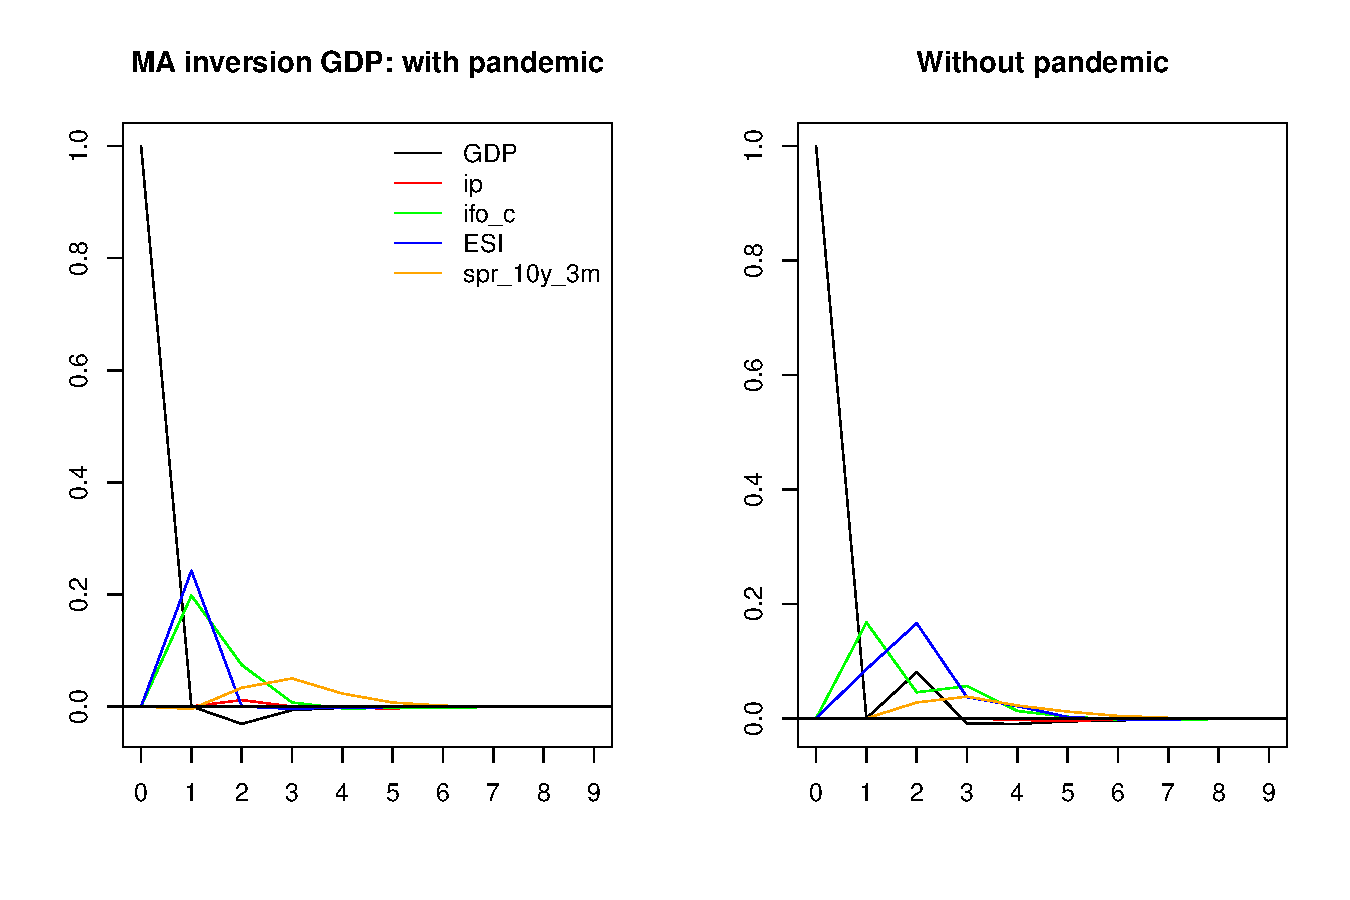
\includegraphics[height=3in, width=6in]{./Figures/ma_inv_BIP.pdf}\caption{MA inversion of VAR(1) for GDP: with pandemic (left) and without pandemic (right).\label{ma_inv_BIP}}\end{center}\end{figure}


The model summarizes key features of the data, where lagging series (GDP and industrial production, when accounting for publication lags) depend on  indicators leading in relative terms. In particular, the impulse response of the spread (rightmost panel in the figure) suggests the relevance of a univariate model for this specific leading indicator.


\section{Direct Forecasts}\label{direct_forecast}

\subsection{`Classic' Direct Forecast}\label{cdf}

So-called direct forecasts are obtained by regressing the relevant indicators on forward-shifted BIP, accounting for the additional publication lag. For illustration of the concept, we here rely on all indicators and full sample information, excluding the pandemic. In-sample forecasts and the shifted BIP, which serves as the target, are presented in Figs. \ref{direct_wc} (full dataset without the pandemic) and \ref{direct_wc_financial_crisis} (financial crisis) for horizons up to three quarters ahead. 
\begin{figure}[H]\begin{center}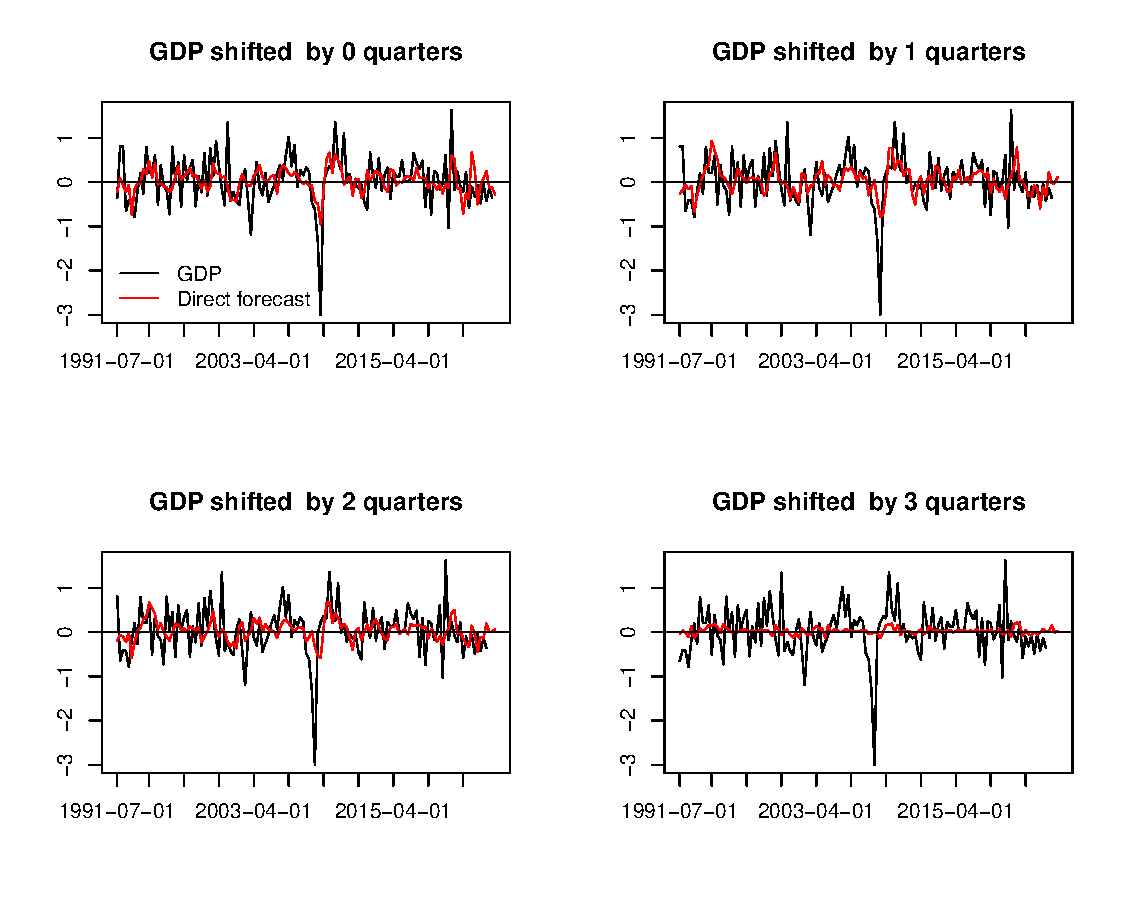
\includegraphics[height=5in, width=6in]{./Figures/direct_wc_all.pdf}\caption{Direct forecasts (red lines) based on all indicators and full sample information, without the pandemic: GDP (black line) shifted by zero one, two and three quarters.\label{direct_wc}}\end{center}\end{figure}\begin{figure}[H]\begin{center}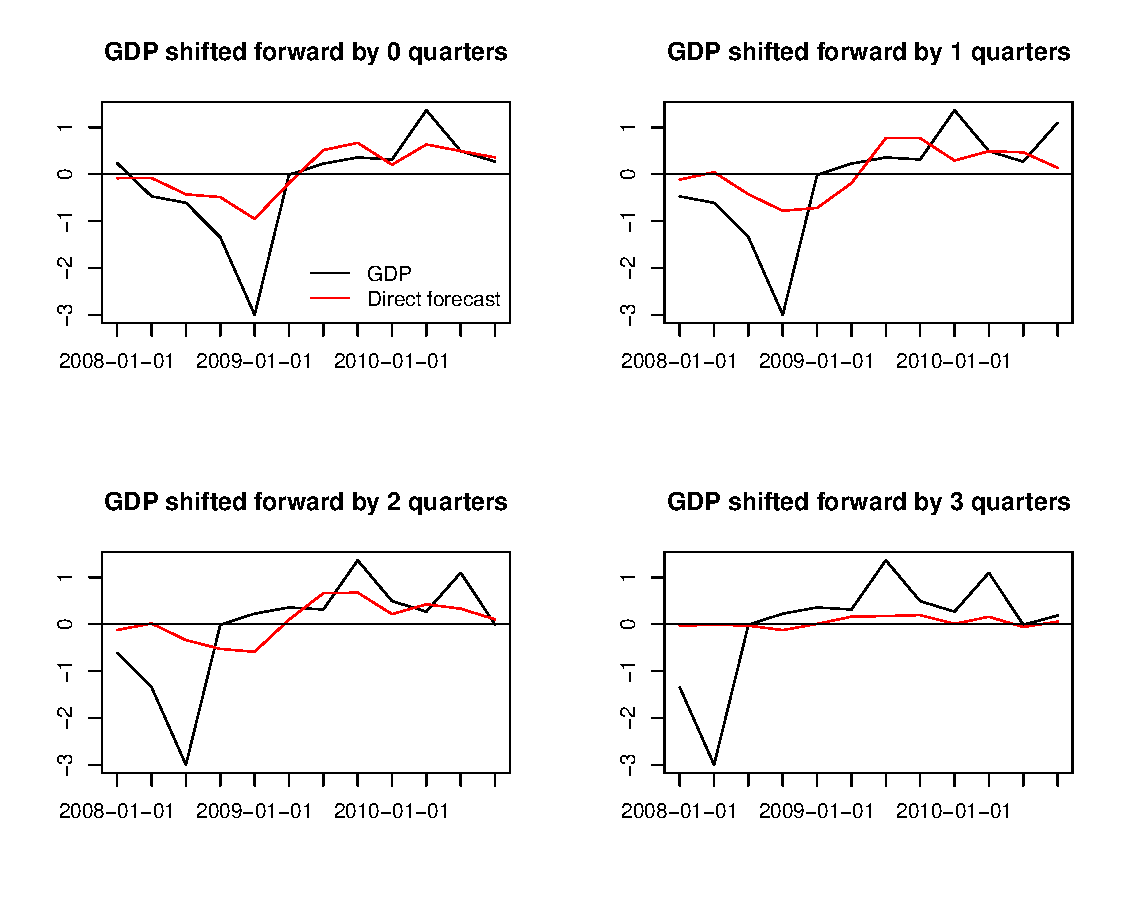
\includegraphics[height=5in, width=6in]{./Figures/direct_wc_financial_crisis.pdf}\caption{Direct forecast  across the financial crisis:  regression based on all indicators and full sample information, without the pandemic.\label{direct_wc_financial_crisis}}\end{center}\end{figure}The results indicate that as $h$ increases, the peaks and dips of the direct forecasts become increasingly right-shifted (delayed) relative to the target. Additionally, the F-statistics precipitously decline from $F=3.21$, for $h=2$, to $F=0.28$, for $h=3$, see Table \eqref{f_stat}, suggesting that the predictor becomes statistically insignificant for larger forecast horizons exceeding two quarters (link to Heinisch and Scheufele).   


\subsection{Filter: HP(160)}

As shown, the performance of direct forecasts sharply declines for larger forecast horizons. We conjecture that erratic short-term fluctuations -—unpredictable high-frequency noise -— overlay the data, thereby obscuring the effective 'signal' and making a direct regression more susceptible to overfitting. We therefore envisage to highlight the signal by applying a filter to dampen high-frequency noise. 
The so-called Hodrick-Prescott filter is a classic tool used in business cycle analysis: the filter is specified by a single smoothing parameter $\lambda$ and the value $\lambda=1600$ is specifically recommended for quarterly data. However, Phillips and Jin (2021) suggest that the HP(1600) filter removes relevant information due to excessive smoothing.  In our context, this oversmoothing issue would be further exacerbated when considering forecast horizons shorter than a year -—an interval inconsistent with the mean duration of up to several years of business cycles, as highlighted by the HP(1600). Consequently, we here select a more adaptive HP(160) 'target' filter. 
While this choice may appear somewhat arbitrary, an analysis of the filter in the frequency domain confirms a more suitable profile for the corresponding amplitude function, assigning greater weight to yearly components -—relevant in our prediction framework-— than the classic quarterly HP filter. This approach also addresses and controls for undesirable high-frequency noise. See Fig. \ref{hp_160}, which presents both two-sided and (classic) one-sided filters (top panels) along with the associated amplitude functions (bottom panels). We now posit the HP(160) filter as a means to achieve better forecasting performance at larger horizons, noting that a comprehensive technical analysis of the effect of $\lambda$ on the resulting BIP predictor can be conducted using the M-SSA package. 
\begin{figure}[H]\begin{center}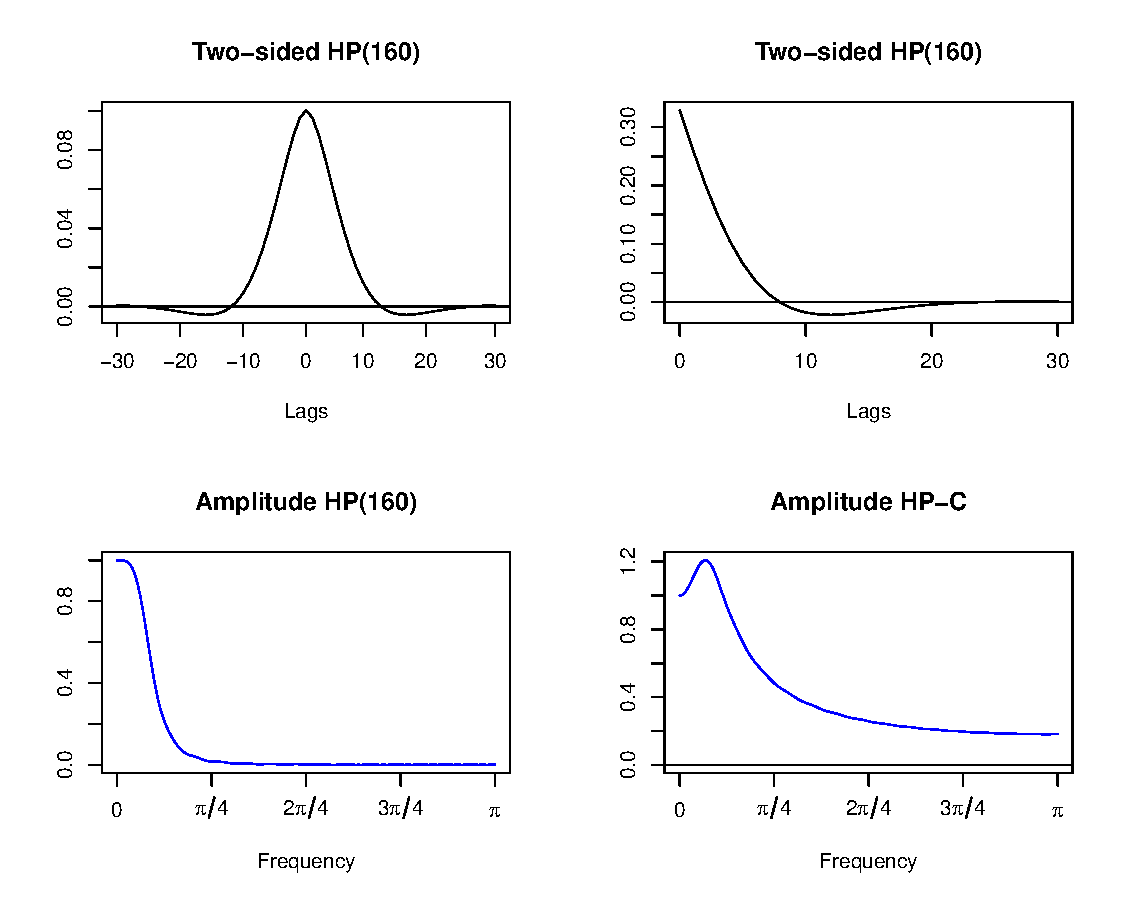
\includegraphics[height=5in, width=6in]{./Figures/hp_160.pdf}\caption{Two-sided HP-160) (top left) and one-sided (concurrent) HP-C filters (top right) with corresponding amplitude functions (bottom).\label{hp_160}}\end{center}\end{figure}
\subsection{Direct HP Forecast}\label{hpdf}


Extending the `classic' direct forecast design, we here consider filtered indicators, based on the one-sided HP(160), denoted as HP-C: the filtered indicators are explanatory variables for the regressions on forward-shifted BIP\footnote{Katja and Simon: for each forecast horizon $h=0,1,2,3$ I'm using corresponding forecasts of the real-time filter output, assuming the data to be white noise (assuming an ARMA model does not lead to significantly different results). I think we might ignore these technical details in the paper.}. As in the previous section, we rely on all indicators as well as the full sample estimate for illustration, see Figs.\eqref{direct_hp_forecasts} (all observations with exclusion of the pandemic) and \eqref{direct_hp_forecasts_financial_crisis} (financial crisis). A comparison with the classic direct forecasts in Fig.\eqref{direct_wc_financial_crisis} indicates that the new predictors are slightly less retarded (`faster'). 
\begin{figure}[H]\begin{center}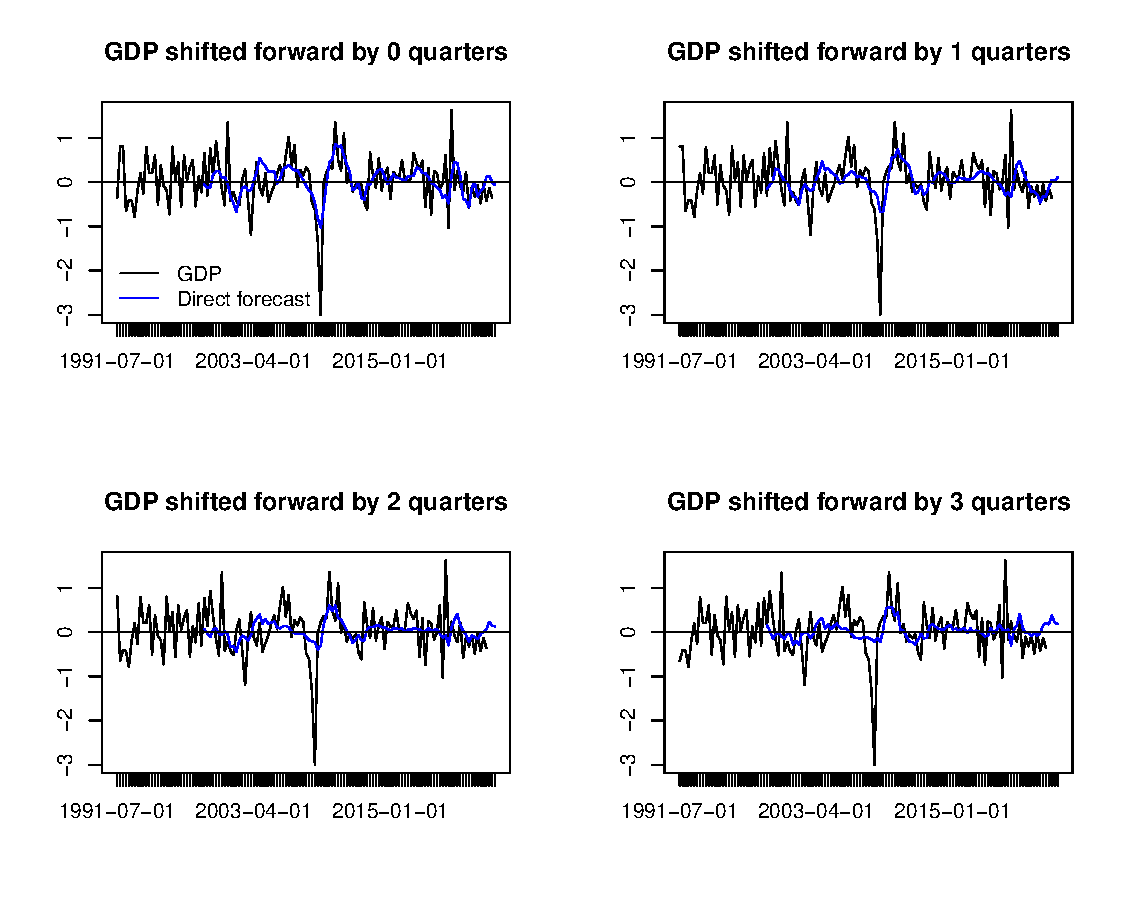
\includegraphics[height=5in, width=6in]{./Figures/direct_hp_forecasts.pdf}\caption{Direct HP forecasts: entire data set with exclusion of the pandemic.\label{direct_hp_forecasts}}\end{center}\end{figure}\begin{figure}[H]\begin{center}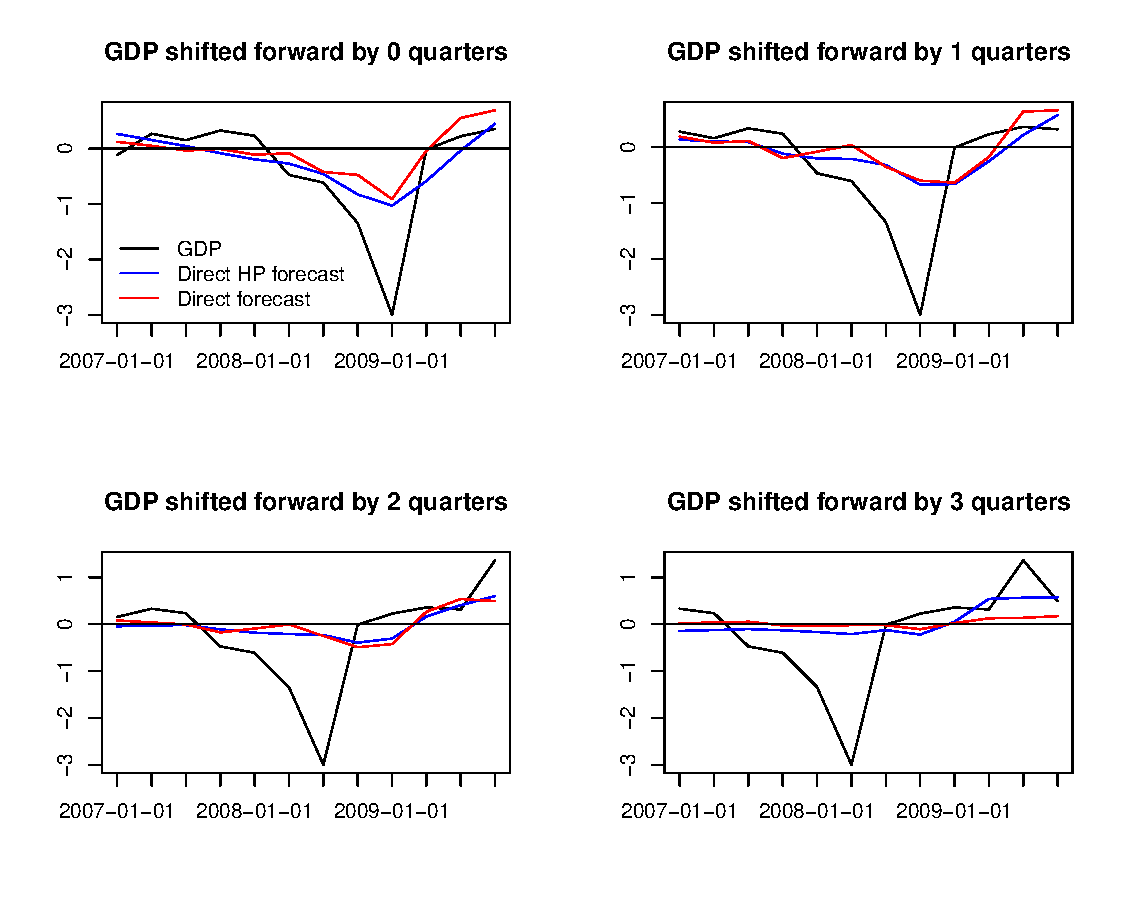
\includegraphics[height=5in, width=6in]{./Figures/direct_hp_forecasts_financial_crisis.pdf}\caption{Shifted GDP (black), direct HP forecast (blue) and classic direct forecast (red) over the curse of the financial crisis:  regression based on all indicators and full sample information (without pandemic).\label{direct_hp_forecasts_financial_crisis}}\end{center}\end{figure}Moreover, the F-statistics are larger than for the direct forecasts, see Table \eqref{f_stat}, but the predictor remains statistically insignificant at forecast horizons exceeding two quarters (even though the evaluation is conducted in-sample and based on all available indicators). 






% latex table generated in R 4.2.2 by xtable 1.8-4 package
% Fri May 23 08:04:53 2025
\begin{table}[ht]
\centering
\begin{tabular}{rrrrrrrr}
  \hline
 & h= 0 & h= 1 & h= 2 & h= 3 & h= 4 & h= 5 & h= 6 \\ 
  \hline
HP-C filtered & 0.000 & 0.001 & 0.036 & 0.046 & 0.049 & 0.012 & 0.022 \\ 
  Unfiltered & 0.028 & 0.000 & 0.001 & 0.910 & 0.509 & 0.091 & 0.178 \\ 
   \hline
\end{tabular}
\caption{Statistical significance of unfiltered and HP-C filtered forecasts based on HAC-adjusted Wald test: all indicators and full sample (without pandemic).  } 
\label{f_stat}
\end{table}
We now propose a more refined causal filter design aiming for statistical significance of the resulting predictor at longer forecast horizons, out-of-sample.   




\section{Multivariate Causal Filter: M-SSA}

The application of the one-sided HP-C filter to the indicators has demonstrated improvements in forecast performance. However, the univariate nature of this filter limits its ability to leverage information from the cross-section, as supported by leading indicators. Additionally, the noise suppression capability of the one-sided filter is compromised, as illustrated by high-frequency leakage of the amplitude function in Fig. \eqref{hp_160} and further elaborated upon by Wildi (2025). To address these limitations, we propose an extension of the Smooth Sign Accuracy (SSA) framework introduced by Wildi (2025).


\subsection{Optimization criterion}



Let $\mathbf{X}_t$ (of dimension $t\times n$) denote a set of $n$ explanatory series $\mathbf{x}_{1t},...,\mathbf{x}_{nt}$, with observations $\mathbf{x}_{it}=(x_{i1},...,x_{it})'$. Let $\mathbf{z}_t=(z_{1},...,z_t)$  denote a target series, which typically lies outside the linear space spanned by $\mathbf{X}_t$  (and is unknown at time $t$). For simplicity, we assume stationarity of all time series involved. In this framework, $\mathbf{X}_t$ corresponds to a matrix of selected economic indicators with $n=5$, and $z_{it}$   is the output of a two-sided HP(160) filter applied to the $i$-th indicator, $i=1,...,5$. Since $z_{it}$  depends on future observations $x_{it+1},x_{it+2},...$, the prediction task involves `tracking' $z_{it}$  using the estimate $y^i_{t}=\sum_{j=1}^ny^i_{jt}$, where $y^i_{jt}=\mathbf{b}^i_j~'\mathbf{x}_{jt}=\sum_{k=0}^{L} b^i_{jk}x_{jk}$ are the outputs of a multivariate (causal or one-sided) filter $\mathbf{B}^i$, with columns $\mathbf{b}^i_{j}$ of fixed length $L$, $j=1,...,5$, assigning weight to the last $L$ observations of the $j$-th indicator $\mathbf{x}_{jt}$ (the fixed-length assumption is merely used for ease of exposition).
For the sake of clarity, we now omit the upper-case index  $i$ for all variables, assuming $z_t=z^{i_0}_{t}$ for some fixed $i_0$.% Additionally, we assume a fixed filter length $L$, such that $\mathbf{B}^i_t=\mathbf{B}_t=\mathbf{B}$, which has dimension $L\times 5$. 
The task of `tracking'  a target can be formalized in different ways; here, we focus on the target correlation $\rho(z,y,h)$ between $y_t$ and $z_{t+h}$, where $h\geq 0$ denotes the forecast horizon (backcasting with $h<0$ is ignored in this context). To streamline the notation and avoid unnecessary complexity, we assume a fixed horizon, say $h=h_0$, so that we may drop the reference to $h$ in our notation. In the univariate case ($n=1$), Wildi (2025) proposes the Simple Sign Accuracy (SSA) as an optimization criterion for this task:
\begin{eqnarray}\label{critssa}
\left.\begin{array}{c}\rho(z,y)\to\max\\
\rho(y,1)=\rho_1\end{array}\right\}.
\end{eqnarray}
Objective function and constraint are expressed in terms of correlations, namely the target correlation $\rho(z,y)$ between target and predictor and the lag-one autocorrelation $\rho(y,1)$ of the predictor. The parameter $\rho_1$ governs the smoothness of the predictor: higher values of $\rho_1$ generally promote smoother trajectories of $y_t$. Formally, assuming that the process $x_t$ is centered (zero-mean), Wildi (2024) establishes a connection between $\rho(y,1)$ and the expected duration between consecutive zero-crossings (sign changes) of $y_t$, the so-called holding time, denoted by $ht(y)$:
\begin{eqnarray*}\label{ht}
ht(y)=\frac{\pi}{\arccos(\rho(y,1))}.
\end{eqnarray*}
Since the non-linear transformation involved is strictly monotonic, the SSA criterion can be reformulated as the optimization problem:
\begin{eqnarray}\label{critssaht}
\left.\begin{array}{c}\rho(z,y)\to\max\\
\frac{\arccos(\rho(y,1))}{\pi}=1/ht_1\end{array}\right\},
\end{eqnarray}
where the smoothness parameter $1/ht_1$ expresses the rate of zero-crossings of the predictor\footnote{Formally, the exact relationship between the zero-crossing rate and the lag-one autocorrelation of the predictor assumes Gaussian time series, but Wildi (2024) demonstrates robustness to deviations from this assumption.}. \\


We now briefly discuss some implications of criterion \eqref{critssaht}. First, the objective function is indifferent to an affine transformation of the predictor. This ambiguity can be resolved by assuming an arbitrary scale and level for $y_t$ (standardization). Alternatively, a mean-square error norm (MSE) may be substituted for the target correlation, as noted in Wildi (2025). In this case, the classic MSE predictor $y_{t,MSE}$ is obtained as a solution to the SSA criterion by insertion of $1/ht_1:=1/ht_{MSE}$ in the constraint, where $ht_{MSE}$ represents the holding time of $y_{t,MSE}$. %If the MSE predictor is noisy, which is often the case in applications, one can select $ht_1>ht_{MSE}$  in the constraint to address the rate of noisy crossings or false alarms. 
Second, the concept can be extended to a multivariate framework, denoted as M-SSA, by generalizing the correlation functions, as detailed in Wildi (2025b). Lastly, sign changes in trend growth, represented by zero-crossings of the target $z_t$, are indicative of relevant changes in the trajectory of the economy, for example at transitions between expansions and recessions. Unfortunately, classic predictors often generate excessively many false `noisy' crossings, due to high-frequency leakage as illustrated by the amplitude function in Fig. \eqref{hp_160} (bottom right panel) and further elaborated upon by Wildi (2025). The SSA criterion helps control this phenomenon. More precisely, Wildi (2025) derives an equivalent dual formulation of criterion \eqref{critssaht}, which distinguishes the SSA solution as exhibiting the smallest rate of zero-crossings of any (linear) predictor with the same target correlation. We now rely on the M-SSA criterion to derive a `smooth' predictor $y_t$ of $z_t$. %In a second stage, serving as a generalization and refinement of the univariate HP-C utilized in the direct HP forecast.


\subsection{M-MSE and M-SSA Nowcasts}

For illustration, we consider a nowcast of the target $z_t$ generated by the output of the two-sided HP(160) filter applied to BIP, which we denote by HP-BIP. We compare the classic multivariate mean squared error (MSE) predictor, denoted by M-MSE, with the M-SSA predictor, where we set $ht_1=1.5ht_{MSE}$ in the holding time constraint. This configuration ensures that the M-SSA predictor produces approximately 33$\%$ fewer zero-crossings than M-MSE over the long term. The purpose of this constraint is to compare the effect of a different level of smoothness on the prediction performance (target correlation). The estimation of the underlying VAR(1) model employed for the M-MSE and M-SSA is based on data observations up to January 2008. This approach ensures a lengthy out-of-sample period that encompasses significant events such as the financial crisis, the sovereign debt crisis, and the COVID-19 pandemic. Further details and background information are available in Wildi (2025b). All computations are performed utilizing the M-SSA package, as documented in Wildi (2025b).\\

Figure \ref{bk_gammak} displays the coefficients of the multivariate nowcasts, where increased smoothing achieved through the M-SSA method manifests as a distinct pattern in the filter weights, notably influencing the rate of decay across increasing lags. The resulting filtered series, presented in Figure \ref{mssa_msse_now}, are standardized to enable direct comparisons. The M-SSA nowcast adheres to the specified constraint, exhibiting approximately one-third fewer zero-crossings than the M-MSE, confirming the effectiveness of the smoothness control imposed during the design. This is further corroborated by Table \ref{corhtnow}, which reports empirical holding times and target correlations. Increased smoothness achieved by the M-SSA comes at the cost of a slight reduction in tracking accuracy, as indicated by a marginally lower target correlation. This highlights the inherent trade-off—often referred to as the prediction dilemma—between smoothness (zero-crossing rate) and predictive accuracy (target correlation) within the M-SSA criterion.
\begin{figure}[H]\begin{center}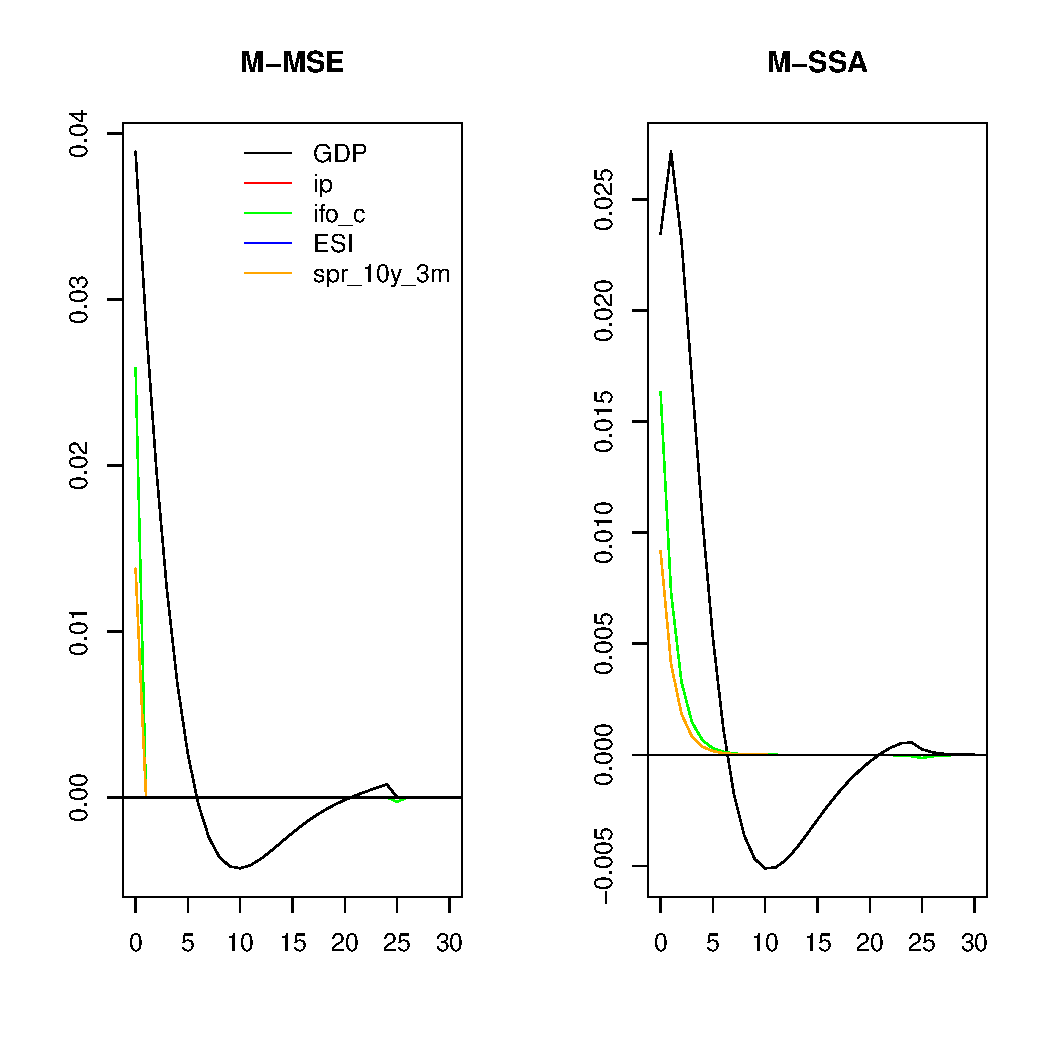
\includegraphics[height=3in, width=5in]{./Figures/bk_gammak.pdf}\caption{Multivariate M-MSE (left) and M-SSA  (right) nowcast filters.\label{bk_gammak}}\end{center}\end{figure}\begin{figure}[H]\begin{center}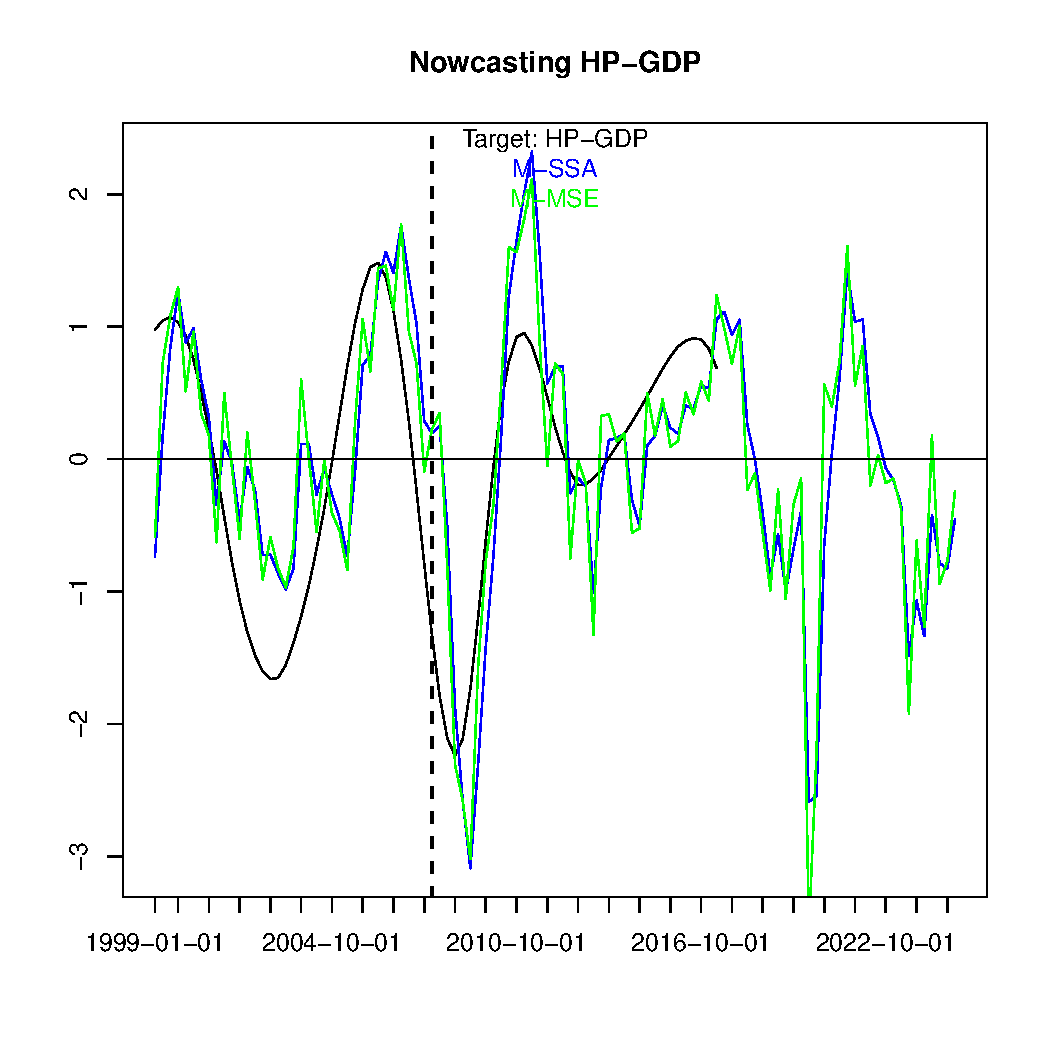
\includegraphics[height=4in, width=5.5in]{./Figures/mssa_msse_now.pdf}\caption{Two-sided HP(160) applied to GDP (target, black) and nowcasts:  M-SSA (blue) and  M-MSE (green). The dashed vertical line delimits in- and out-of-sample spans. The two-sided filter does not extend to the sample end.\label{mssa_msse_now}}\end{center}\end{figure}% latex table generated in R 4.2.2 by xtable 1.8-4 package
% Fri May 23 08:05:05 2025
\begin{table}[ht]
\centering
\begin{tabular}{rrr}
  \hline
 & M-SSA & M-MSE \\ 
  \hline
Target correlation & 0.68 & 0.69 \\ 
  HT & 6.50 & 3.71 \\ 
   \hline
\end{tabular}
\caption{Sample target correlations and HTs of M-SSA and M-MSE nowcasts.  } 
\label{corhtnow}
\end{table}The results validate that the smoothing constraint incorporated into the multivariate extension of Criterion \eqref{critssa} effectively manages the zero-crossings of the predictor: sample estimates of the holding times (HTs) align with the expected values derived from Equation \eqref{ht}\footnote{Effective convergence of sample estimates to their theoretical expected values —assuming the true data-generating process is known— can be validated using the M-SSA package. This validation is typically performed through analyses of very long samples of simulated (multivariate) data, ensuring the consistency of the estimation procedures under idealized conditions.}. An increase of $50\%$ in the HT relative to the M-MSE predictor has only a modest effect on the target correlation, suggesting that this tradeoff could be beneficial in our application. Going forward, we now omit the M-MSE, as it is a special case of the more general M-SSA framework.


\subsection{M-SSA Forecasts}

The previously described nowcast example can be systematically extended to generate forecasts of the target variable. This extension utilizes the same empirical framework, incorporating an assumed $50\%$ increase in the HT over the M-MSE, and considers forward shifts of $h=0,...,6$  quarters of HP-BIP (note that M-SSA does not target BIP explicitly). %This approach facilitates the assessment of forecast performance across multiple horizons within the established methodological context. 
The influence of the forecast horizon on the M-SSA design is depicted in Fig. \eqref{bk_h}, which contrasts nowcast and one-year-ahead forecast: as $h$ increases (right panel), the scaling factor diminishes (zero-shrinkage), attributable to increased forecast uncertainty, and there is a relative amplification of the influence of the relevant indicators, leading BIP in relative terms.Additionally, a phase shift associated with the filter applied to BIP is observed (red line, right panel), reflecting the cyclical characteristics inherent to the HP filter. While this phase effect might cause an effective sign change in the BIP filter output as $h$ increases—something to be avoided in this context—the low-pass filters assigned to the additional 'leading' indicators (green and violet lines, right panel) continue to effectively track the low-frequency components of HP-BIP. The combination of the phase effect, applied to BIP, and level-tracking through these additional indicators enables more refined and effective tracking of the target compared to univariate forecasts, which rely solely on the phase-effect of the filter to look ahead of time.\\

M-SSA predictors are compared to the traditional univariate HP-C in Figs. \eqref{multivar_vs_univar} and \eqref{mssa_hpc_financial_crisis}. In the first figure, we compare both filters across the periods of the financial crisis (top panels) and the COVID-19 pandemic (bottom panels), for forecast horizons $h=0,...,6$. The nowcast from the previous section is included for reference. In the second figure we compare both filters to the forward-shifted BIP for shifts larger than two quarters. All series are standardized to facilitate visual comparison. The primary distinction of the M-SSA approach is the progressive left-shift of the predictor as a function of $h$; this shift becomes more pronounced with increasing $h$ and appears to be consistent across all levels, including the peaks and troughs of the series. Conversely, the positions of peaks and troughs in the HP-C series appear to remain largely unaffected by variations in $h$. The more pronounced and systematic left-shift observed in the M-SSA forecasts can be partly attributed to the increasing weight assigned to the additional indicators leading BIP, which dominate the BIP component at larger forecast horizons. %In comparison, the effect of phase shifts—arising from the cyclical nature of the HP-filter and manifesting in the HP-C forecasts (shown in the left panels)—seems less systematic. 
\begin{figure}[H]\begin{center}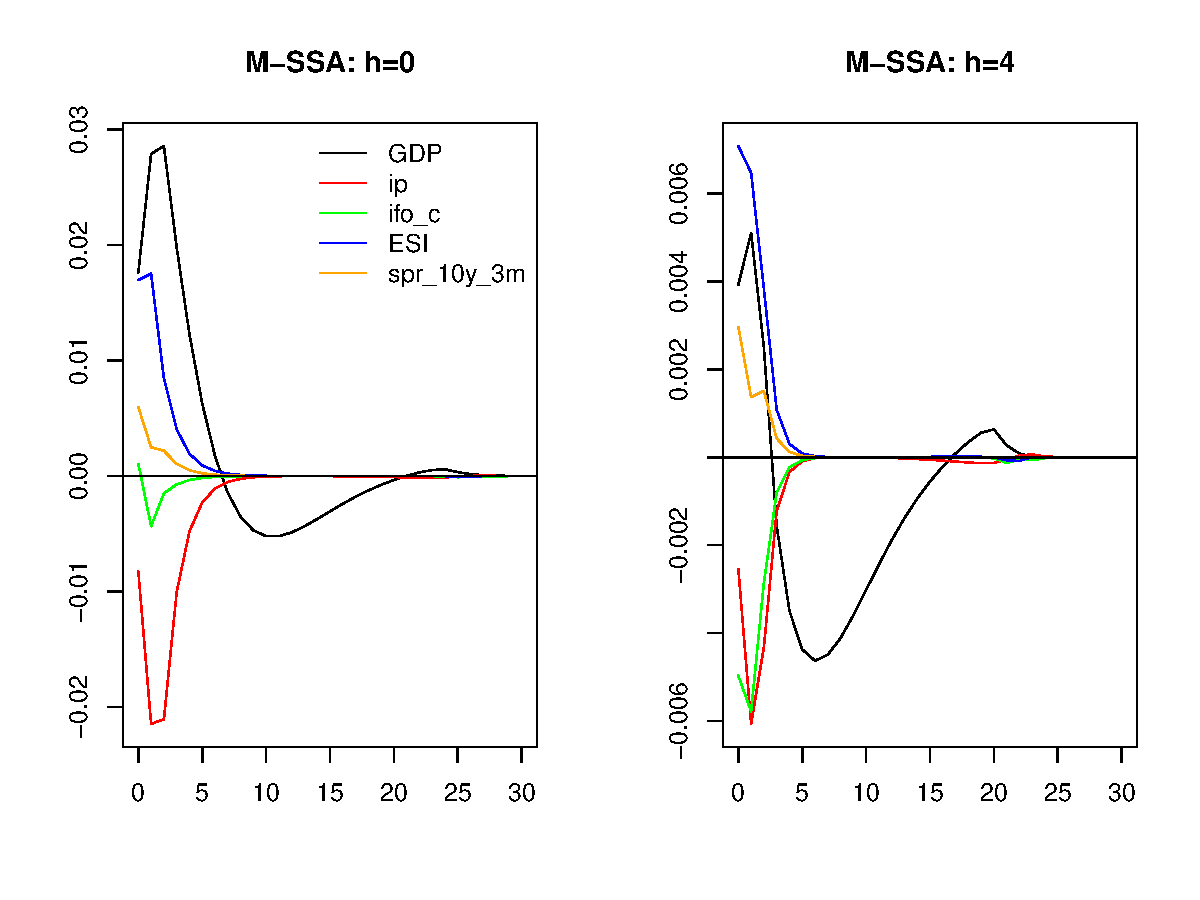
\includegraphics[height=3in, width=5.5in]{./Figures/bk_h.pdf}\caption{Multivariate M-SSA: $h=0$ (nowcast, left) and $h=4$ (one year forecast, right).\label{bk_h}}\end{center}\end{figure}\begin{figure}[H]\begin{center}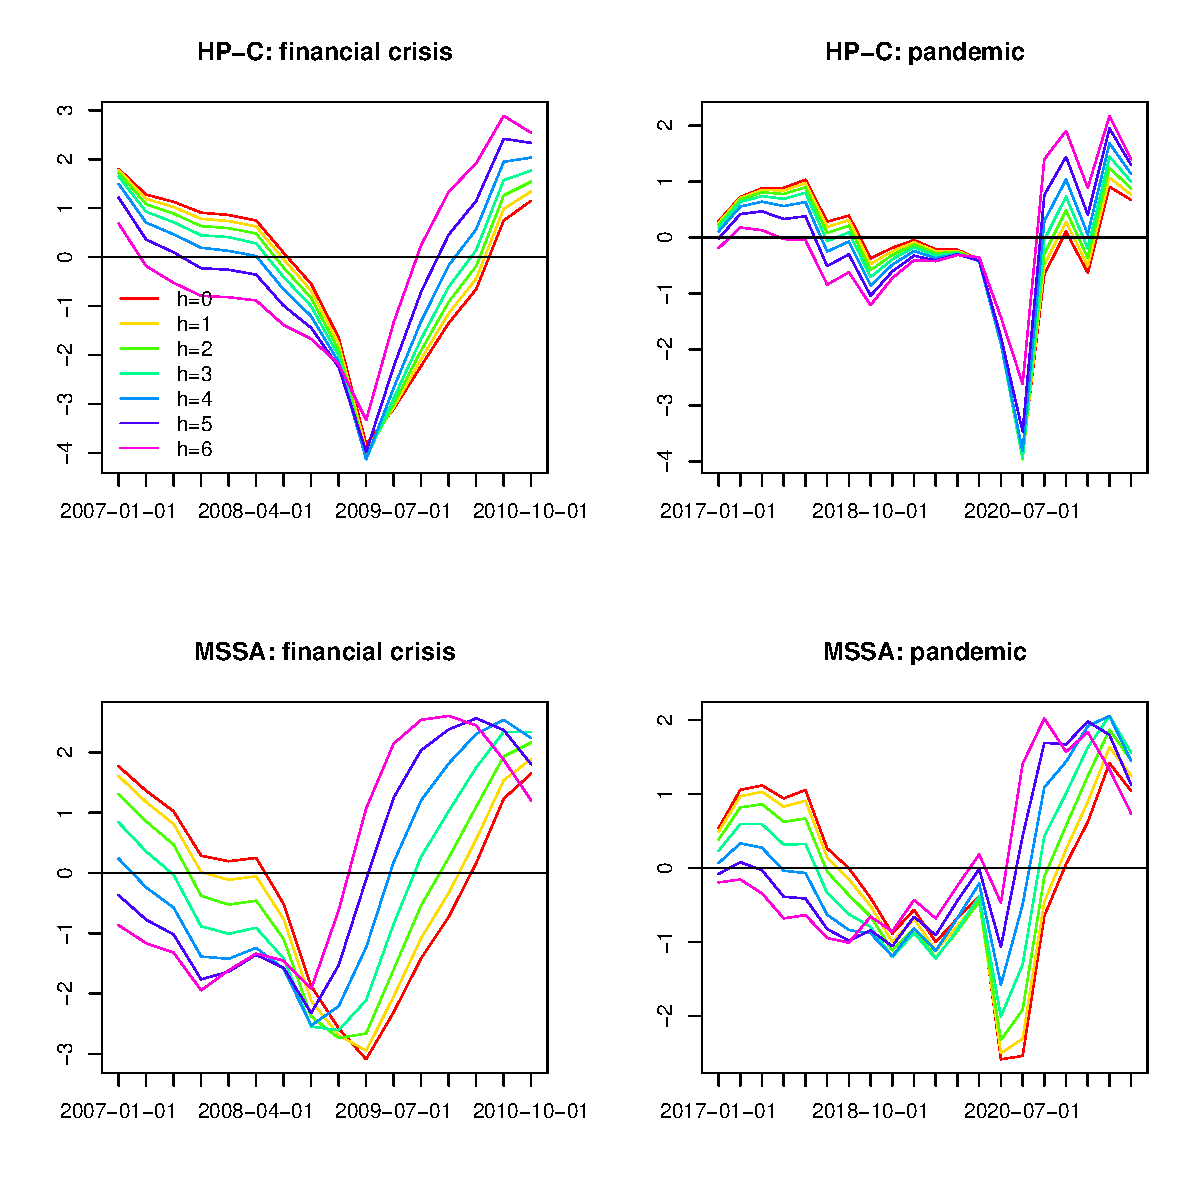
\includegraphics[height=4in, width=5.5in]{./Figures/multivar_vs_univar.pdf}\caption{Now- and forecasts of HP-GDP for $h=0,...,6$: HP-C (top) vs. M-SSA (bottom) across the financial crisis (left) and the pandemic (right).\label{multivar_vs_univar}}\end{center}\end{figure}
\begin{figure}[H]\begin{center}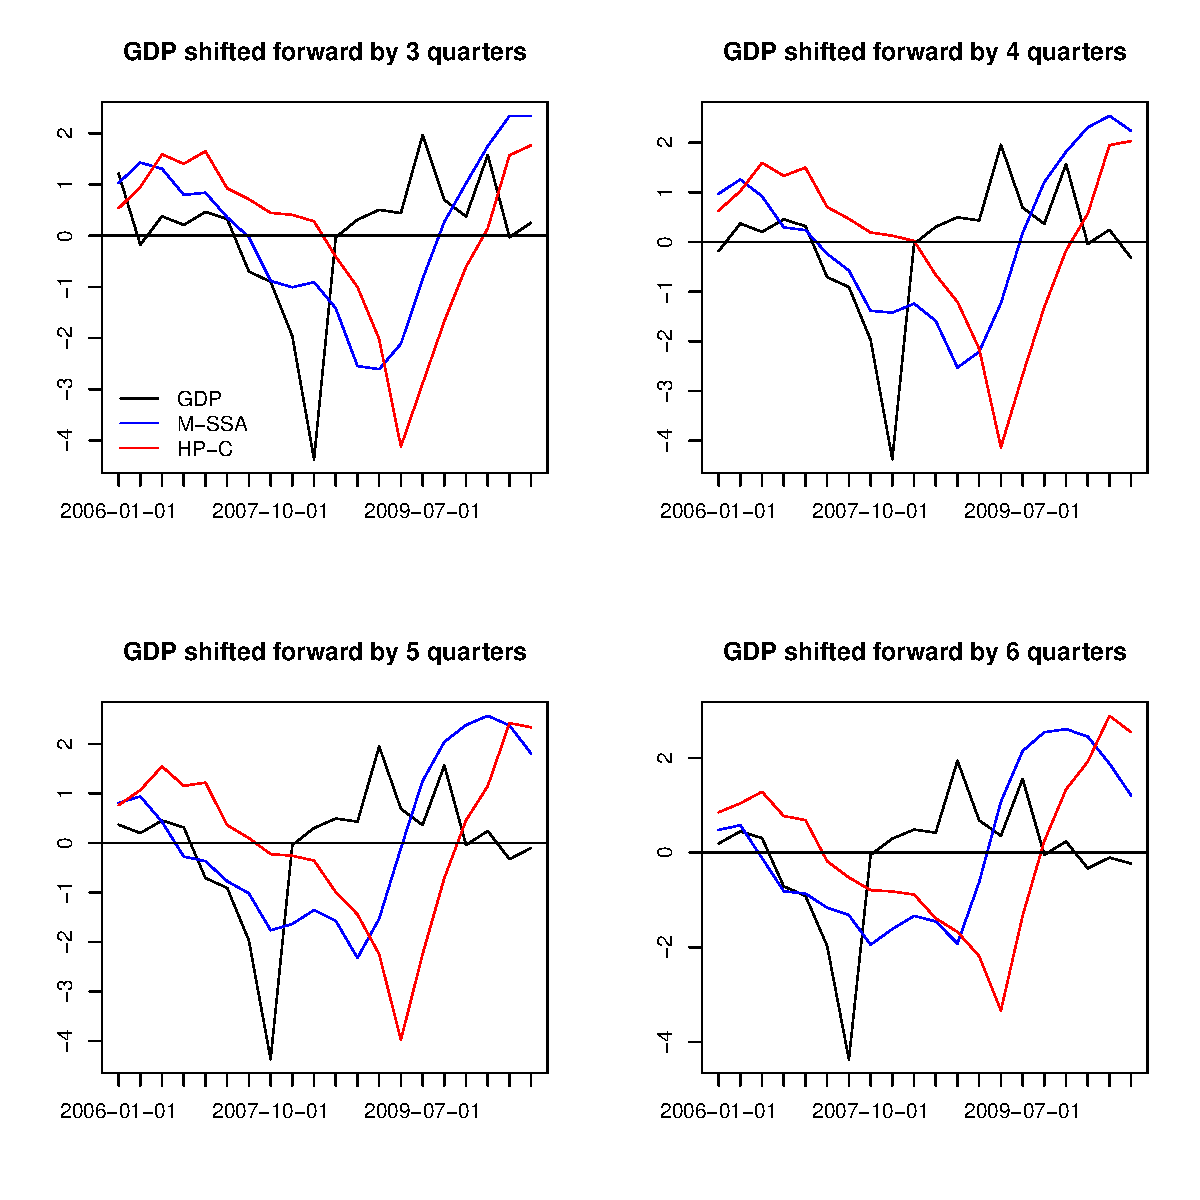
\includegraphics[height=4in, width=5.5in]{./Figures/mssa_hpc_financial_crisis.pdf}\caption{Forward-shifted GDP (black), M-SSA (blue) and HP-C (red) for $h=3,4,5,6$ across the financial crisis. All series are standardized for better visual inspection.\label{mssa_hpc_financial_crisis}}\end{center}\end{figure}

\section{M-SSA Component Predictor}

The targets of the multivariate filters are the smoothed outputs obtained from the acausal two-sided HP(160) filter applied to the five indicators. However, our objective is to develop predictors that emphasize the unfiltered BIP. To achieve this, we can utilize the  M-SSA outputs, referred to as M-SSA components.




\subsection{Standardized Predictor: Equal-Weighting}


Assuming that all M-SSA components contribute equally to BIP prediction, an initial step involves averaging the standardized components to form an equally-weighted composite measure. Subsequently, the predictor is derived by regressing this standardized aggregate on the (forward-shifted) BIP series. Fig. \eqref{mssa_predictor} presents the BIP series alongside the equally-weighted M-SSA predictor. All series are standardized to facilitate visual comparison and to highlight the dynamic shifts, particularly the left-shift characteristic of the predictors.\\

To enhance interpretability and assessment of the M-SSA predictor, we propose analyzing its individual components. For illustration, Fig. \eqref{mssa_predictor_interpretability} shows the nowcast at $h=0$. The solid blue line (the nowcast) approaches the zero line near the end of the sample, with a recent upward movement mainly supported by the leading spread component. In contrast, the ifo- and ESI-components remain near the zero line, while the ip- and BIP-components appear to be awaiting additional evidence and confirmation before signaling a definitive movement.  This type of assessment can be useful for evaluating the relevance of recent changes in the forecasted time series dynamics.
\begin{figure}[H]\begin{center}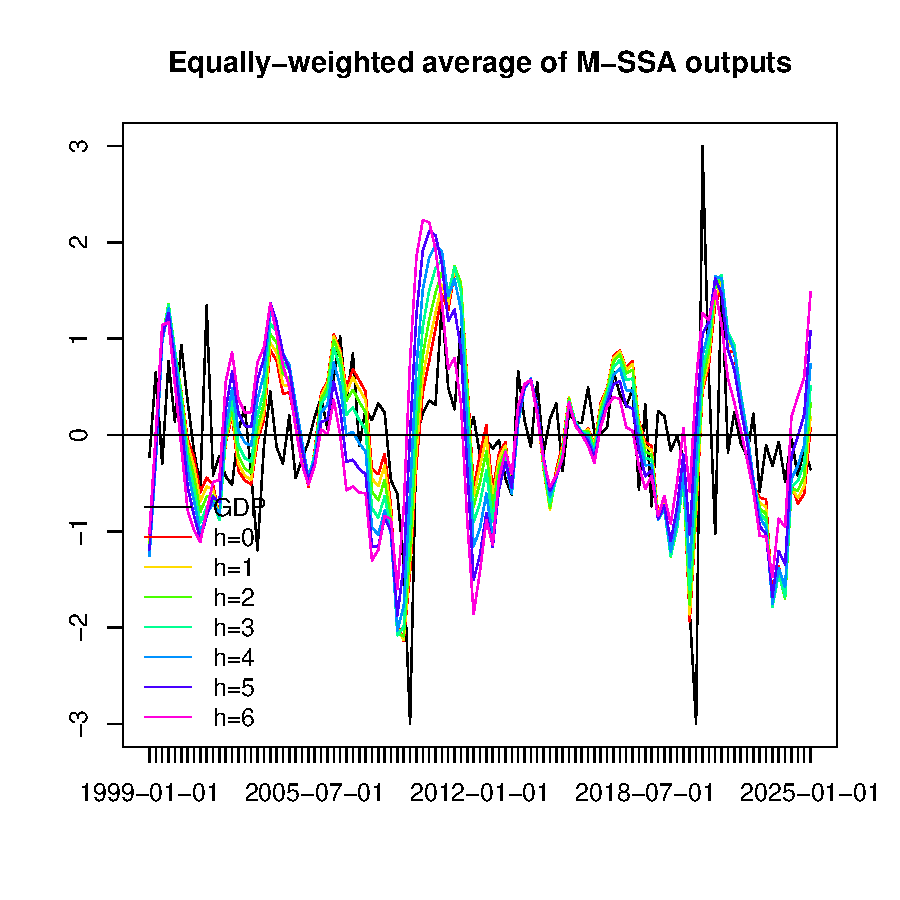
\includegraphics[height=3in, width=4.5in]{./Figures/mssa_predictor.pdf}\caption{BIP and equally-weighted M-SSA predictor: all series standardized.\label{mssa_predictor}}\end{center}\end{figure}\begin{figure}[H]\begin{center}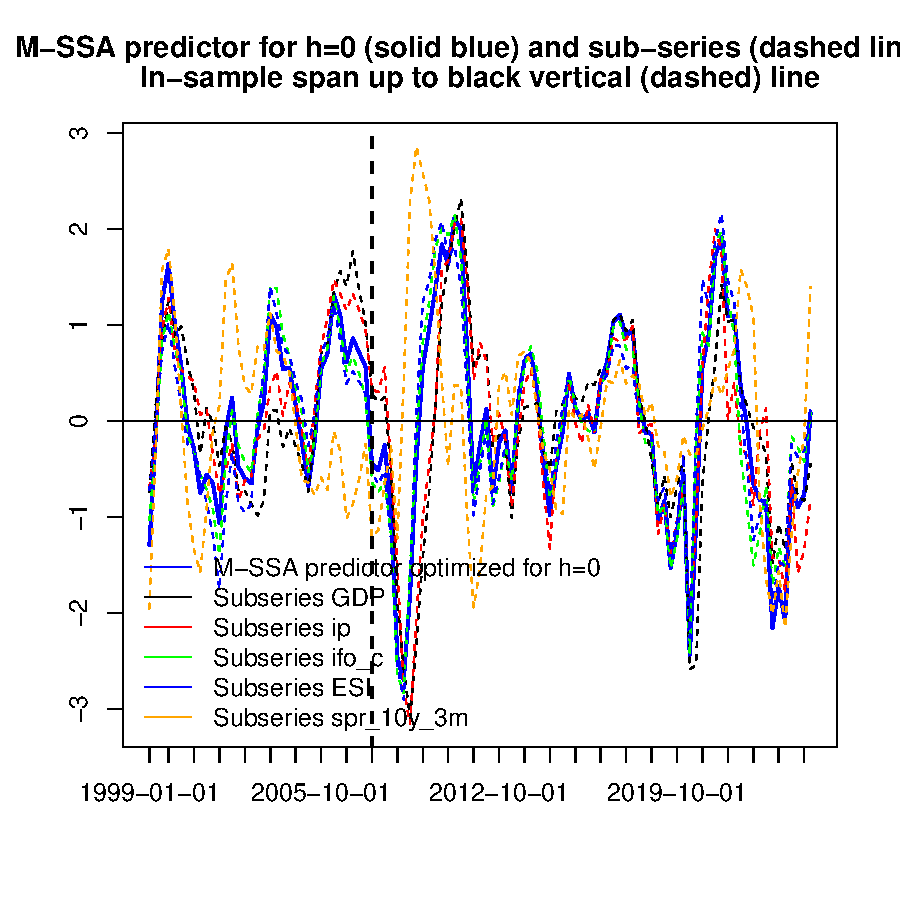
\includegraphics[height=3in, width=4.5in]{./Figures/mssa_predictor_interpretability.pdf}\caption{Equally-weighted M-SSA predictor and M-SSA components: all series standardized.\label{mssa_predictor_interpretability}}\end{center}\end{figure}
%???Eventually add p-values and/rRMSEs???


\subsection{Tracking BIP: Optimal Weighting}


We now utilize the M-SSA components as regressors on forward-shifted BIP, extending the previous (standardized) equally-weighted M-SSA predictor to incorporate optimal weighting of the components. While we keep the M-SSA fixed, as based on data up to January 2008, we implement an expanding window starting from January 2007 for deriving the component weights, which are up-dated on a quarterly basis (this contrasts with Section \eqref{direct_forecast} which was based on the full sample information). \\


There are various combinations of M-SSA components for tracking BIP. For illustration, we here select the single BIP component resulting from the M-SSA filter tracking HP-BIP. Table \eqref{p_val_hpbip_wc} reports HAC-adjusted p-values from regressions of the out-of-sample predictor on HP-BIP, indicating a strong link between the predictor and the target, out-of-sample. 
% latex table generated in R 4.2.2 by xtable 1.8-4 package
% Fri May 23 08:05:56 2025
\begin{table}[ht]
\centering
\begin{tabular}{rrrrrrrr}
  \hline
 & h=0 & h=1 & h=2 & h=3 & h=4 & h=5 & h=6 \\ 
  \hline
Shift=0 & 0.000 & 0.000 & 0.001 & 0.002 & 0.005 & 0.020 & 0.112 \\ 
  Shift=1 & 0.000 & 0.000 & 0.000 & 0.001 & 0.002 & 0.005 & 0.019 \\ 
  Shift=2 & 0.000 & 0.000 & 0.000 & 0.001 & 0.001 & 0.003 & 0.006 \\ 
  Shift=3 & 0.018 & 0.007 & 0.002 & 0.000 & 0.002 & 0.003 & 0.004 \\ 
  Shift=4 & 0.180 & 0.100 & 0.040 & 0.010 & 0.002 & 0.005 & 0.005 \\ 
  Shift=5 & 0.579 & 0.432 & 0.261 & 0.108 & 0.027 & 0.008 & 0.009 \\ 
   \hline
\end{tabular}
\caption{HAC adjusted p-values of regressions of BIP (M-SSA) component optimized for forecast horizons $h=0,...,6$  (the columns) on HP-BIP shifted forward by shift=0,...,5 (the rows). Out-of-sample span starting in Jan-2007, without pandemic.} 
\label{p_val_hpbip_wc}
\end{table}Our choice—focusing on the single M-SSA BIP component—emphasizes simplicity and interpretability, as future BIP and HP-BIP are connected through their shared low-frequency component. Additionally, the M-SSA BIP component is the most important predictor in the regression of the M-SSA outputs on BIP.  Finally, revisions due to quarterly updates of the regression equations are minimized by this predictor, and the estimates are more stable and robust over time\footnote{Other combinations can be experimented with using the M-SSA package. Regression weights of more complex designs, involving multiple components, tend to be more difficult to interpret due to the occurrence of negative weights and potential sign changes of the regressors over time, which may indicate overfitting or non-stationarity.} (see Section \eqref{revisions}). Note that information from the other  indicators is incorporated into the M-SSA BIP component through the multivariate filter design.\\



This setup allows us to evaluate the out-of-sample performance of various predictor approaches, including: (i) the simple mean of BIP, (ii) the direct forecast method described in Section \eqref{cdf}, (iii) the direct HP forecasts from Section \eqref{hpdf}, based on the univariate HP-C, and (iv) the new M-SSA BIP component predictor. %For completeness, we also consider an M-MSE component predictor derived from outputs of the multivariate MSE filter. 





\subsection{Out-of-Sample Forecast Performances}\label{oosp}


Tables \ref{p_val_wc} and \ref{rRMSE_mSSA_comp_mean_wc} present HAC-adjusted p-values and rRMSEs for the GDP component predictor. They are obtained from the simple regressions 

\begin{equation}
    \textrm{GDP}_{t+shift}=\beta_0(shift,h)+\beta_1(shift,h) \cdot \textrm{M-SSA}^{\textrm{GDP}}_t(h) + \epsilon_t^{shift,h}
    \label{eq:GDP_M-SSA}
\end{equation}

where $\textrm{M-SSA}^{\textrm{GDP}}_t(h)$ is the out-of-sample M-SSA predictor for GDP (not HP-GDP.)
%(in contrast to Table \ref{p_val_hpbip_wc}, which emphasized HP-GDP.) 
The p-values test $H_0 : 0 = \beta_1(shift,h)$ and do not account for potential bias or mis-scaling of the GDP predictor. In contrast, the rRMSEs, evaluated against the mean benchmark, incorporate eventual bias and mis-scaling effects. Additional results involving other predictor benchmarks are provided in the appendix, based on data sets with and without the pandemic. \\


The purposes of Equation \ref{eq:GDP_M-SSA} are twofold: first, the regression parameters enable affine transformations of the left-hand side variable, so that the standardized target $\textrm{GDP}_{t+shift}$ can be replaced by the original log-returns without affecting the p-values or rRMSEs reported in Tables \ref{p_val_wc} and \ref{rRMSE_mSSA_comp_mean_wc} (noting that the benchmark predictors, i.e., the direct forecasts and the arithmetic mean, similarly adjust to affine transformations); second, the static scale adjustment by $\beta_1(shift,h)$ compensates for the increasing zero-shrinkage of $\textrm{M-SSA}^{\textrm{GDP}}_t(h)$, reflecting greater uncertainty  as the forecast horizon $h$ increases. This simple transformation allows $\textrm{M-SSA}^{\textrm{GDP}}_t(h)$ to be used as a predictor for $\textrm{GDP}_{t+shift}$ even when $h\neq shift$. Such flexibility enables assessment of the dynamic left-shift of $\textrm{M-SSA}^{\textrm{GDP}}_t(h)$, as illustrated in Figure \ref{{multivar_vs_univar}}, at various forward-shifts of $\textrm{GDP}_{t+shift}$.\\  


When excluding the pandemic, the direct forecasts outperform the mean forecast up to two quarters ahead, see Table \ref{rRMSE_mSSA_direct_mean_without_covid8}.\footnote{However, the pandemic period generally obscures the relationships between predictors and GDP.} However, the M-SSA component predictor, optimized for longer forecast horizons, outperforms the mean benchmark up to 6Q ahead. Additionally, the GDP component predictor optimized for large forecast horizons $h\geq 4$ surpass the direct forecasts for $shift>2$, see Table \ref{rRMSE_mSSA_comp_direct_without_covid7}. Statistical significance of the GDP component predictor, optimized for larger forecast horizons, can be established for at least up to one year ahead.


%???check whether rMSE is decreasing towards sample end (because initial estimate towards 2007 is unreliable)???

% latex table generated in R 4.2.2 by xtable 1.8-4 package
% Fri May 23 08:06:06 2025
\begin{table}[ht]
\centering
\begin{tabular}{rrrrrrrr}
  \hline
 & h=0 & h=1 & h=2 & h=3 & h=4 & h=5 & h=6 \\ 
  \hline
Shift=0 & 0.086 & 0.049 & 0.018 & 0.005 & 0.002 & 0.002 & 0.042 \\ 
  Shift=1 & 0.238 & 0.165 & 0.097 & 0.033 & 0.005 & 0.001 & 0.005 \\ 
  Shift=2 & 0.815 & 0.680 & 0.428 & 0.180 & 0.029 & 0.007 & 0.008 \\ 
  Shift=3 & 0.866 & 0.963 & 0.922 & 0.699 & 0.269 & 0.079 & 0.047 \\ 
  Shift=4 & 0.361 & 0.808 & 0.989 & 0.954 & 0.546 & 0.127 & 0.034 \\ 
  Shift=5 & 0.351 & 0.786 & 0.982 & 0.943 & 0.579 & 0.245 & 0.042 \\ 
   \hline
\end{tabular}
\caption{HAC adjusted p-values of regressions of M-SSA component predictors optimized for forecast horizons $h=0,...,6$  (the columns) on BIP shifted forward by shift=0,...,5 (the rows). Out-of-sample span starting in Jan-2007, without pandemic.} 
\label{p_val_wc}
\end{table}% latex table generated in R 4.2.2 by xtable 1.8-4 package
% Fri May 23 08:06:06 2025
\begin{table}[ht]
\centering
\begin{tabular}{rrrrrrrr}
  \hline
 & h=0 & h=1 & h=2 & h=3 & h=4 & h=5 & h=6 \\ 
  \hline
Shift=0 & 0.950 & 0.917 & 0.877 & 0.851 & 0.865 & 0.910 & 0.960 \\ 
  Shift=1 & 1.028 & 1.007 & 0.960 & 0.899 & 0.867 & 0.878 & 0.912 \\ 
  Shift=2 & 1.040 & 1.043 & 1.030 & 0.984 & 0.933 & 0.910 & 0.913 \\ 
  Shift=3 & 1.006 & 1.024 & 1.040 & 1.025 & 0.983 & 0.952 & 0.941 \\ 
  Shift=4 & 0.977 & 1.003 & 1.034 & 1.040 & 1.005 & 0.964 & 0.937 \\ 
  Shift=5 & 0.984 & 1.011 & 1.044 & 1.057 & 1.031 & 0.986 & 0.949 \\ 
   \hline
\end{tabular}
\caption{rRMSEs of M-SSA components predictor benchmarked against the expanding mean of BIP. Out-of-sample span starting in Jan-2007, without pandemic.} 
\label{rRMSE_mSSA_comp_mean_wc}
\end{table}

\section{Revisions}\label{revisions}



Revisions refer to changes in the historical values of a time series resulting from updates with new information. Revisions of the M-SSA component predictor can arise from data updates, which we do not analyze further here\footnote{Except for BIP, the other indicators are not or only slightly revised. Moreover, the smoothing effect of filters mitigates the effect of revisions when compared to direct forecasts.}, or from updates to predictor parameters. The latter can be further separated into changes in VAR parameters and regression weights. 


\subsection{Revisions: Regression Equation Only}

For illustration, we here focus on a forecast horizon $h=4$ for the BIP component predictor and a forward-shift $shift=4$ for BIP, noting that similar results would be obtained with other combinations of $h$ and $shift$. 
%???Check left-shift of MA-inversion of M-SSA and M-MSE
%??? Check forecast excess for HP-C
%??? Justification HP(160): replace HP(1600) by AR(2) with similar persistency but shorter cycle lengthi, i.e. $a_1=-2"persistency*acos(\theta, a_2=persistency$.
Fig.\eqref{revisions1} compares the final and real-time predictors: as the sample size increases, the real-time predictor converges steadily to the final predictor and the rate of convergence is partially determined by the simplicity of our design, which avoids incorporating additional M-SSA components. 
As a confirmation, Fig.\eqref{revisions2} displays the evolution of the intercept and regression weights over time: with increasing sample size, these estimates seem to converge to fixed points, indicating both the stationarity of the process and the consistency of the estimates (note, however, the slightly elevated values of the regression weight assigned to the M-SSA component during the financial crisis and the pandemic, suggesting a stronger link between the target and the predictor).  In contrast, more complex designs based on multiple M-SSA components can exhibit substantial fluctuations in the regression parameters, sometimes changing signs. This suggests instability and complicates interpretation.
\begin{figure}[H]\begin{center}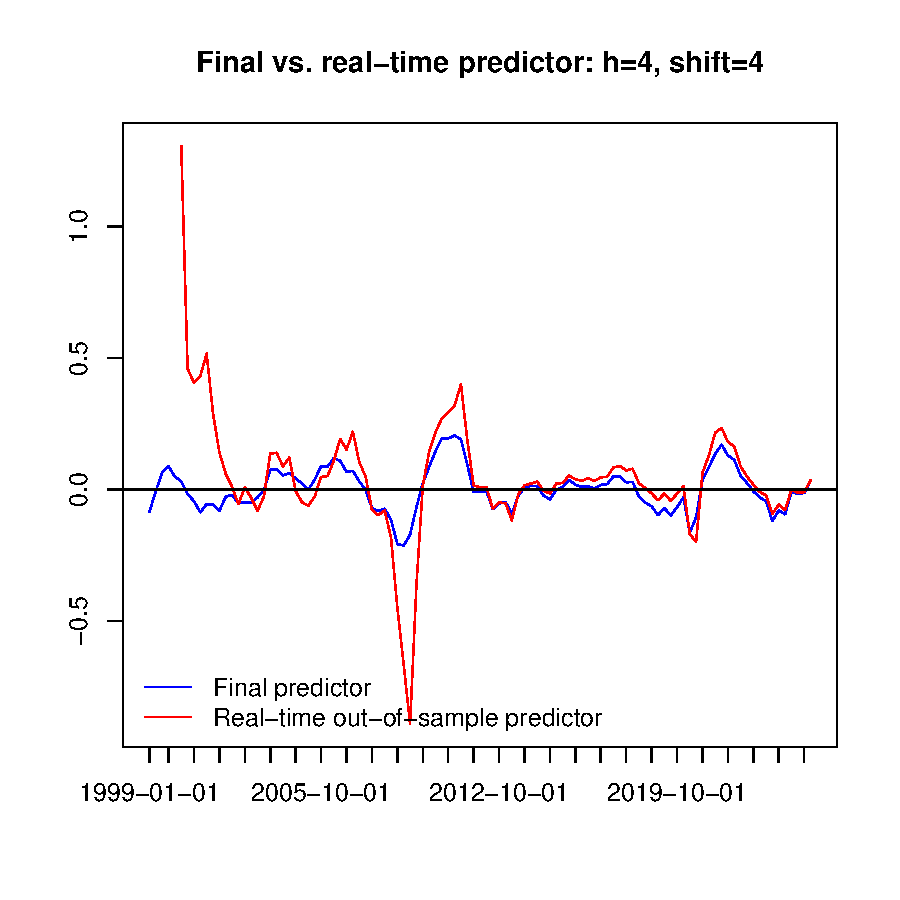
\includegraphics[height=3in, width=4.5in]{./Figures/revisions1.pdf}\caption{Revisions of the M-SSA GDP component predictor are shown, with the final predictor in blue and the real-time design in red. These revisions result from quarterly updates to the regression equations. The M-SSA filter itself remains fixed, based on data up to January 2008.\label{revisions1}}\end{center}\end{figure}\begin{figure}[H]\begin{center}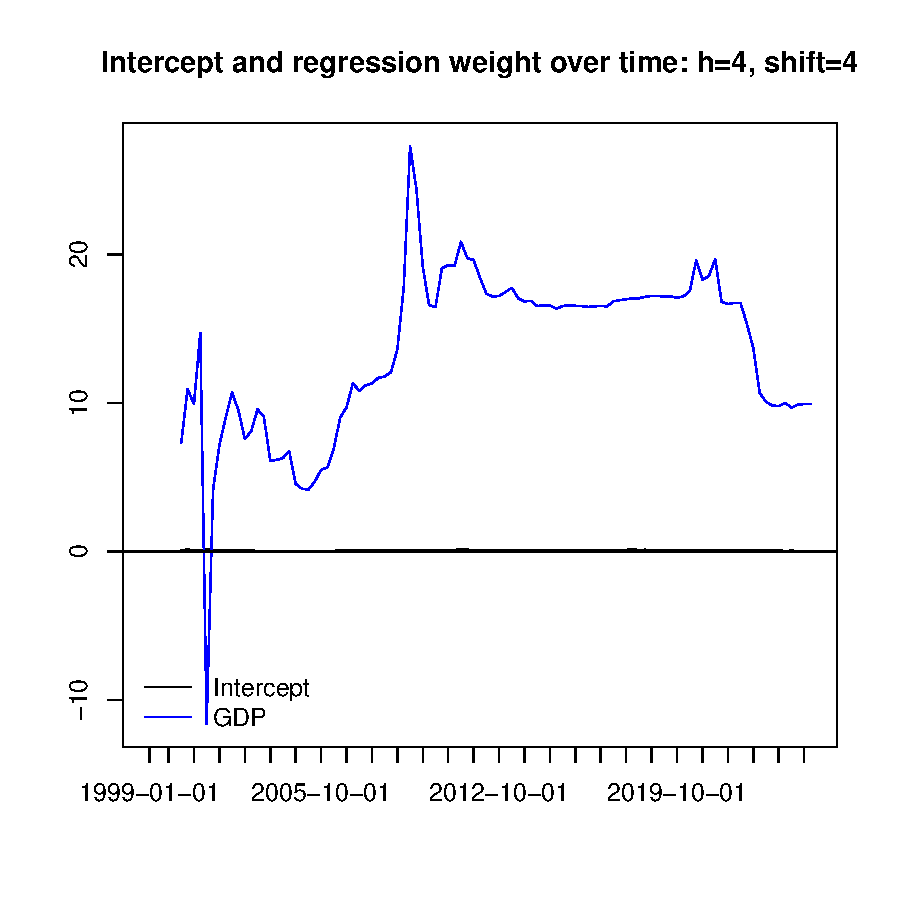
\includegraphics[height=3in, width=4.5in]{./Figures/revisions2.pdf}\caption{Revisions of intercept and regression weight.\label{revisions2}}\end{center}\end{figure}

\subsection{Revisions: M-SSA Only}

The second source of revisions in the M-SSA component predictor arises from updates to the VAR model within the M-SSA filter. We compare the original estimates, based on data up to January 2008, with the final estimates obtained using $h=4$ and $shift=4$ (similar findings apply to other values of forecast horizon and forward-shift).  For consistency, we excluded the entire pandemic episode from the data. Fig.\eqref{up_dated_ma_inv_multi_ip} compares the MA-inversions (impulse responses) of the BIP equation derived from the 'old' and the updated VAR models: unlike the former, the latter incorporates ESI as an additional explanatory variable for BIP. Fig.\eqref{bk_2008_all} illustrates the resulting effect on the M-SSA filter targeting HP-BIP at forecast horizon $h=4$. The updated filter (right panel) assigns more weight to the additional 'leading' indicators relative to BIP. Finally, Fig.\eqref{revisions3} compares the M-SSA BIP predictors. To isolate the effect of the regression revision, the figure displays standardized series. The update to the VAR model influences the left-shift of the predictor (blue line), which appears slightly 'faster' than the original predictor (red line). This suggests that the out-of-sample performance of the M-SSA component predictor may be better than reported in Section \eqref{oosp}, which is based on the fixed and increasingly outdated version of M-SSA.
\begin{figure}[H]\begin{center}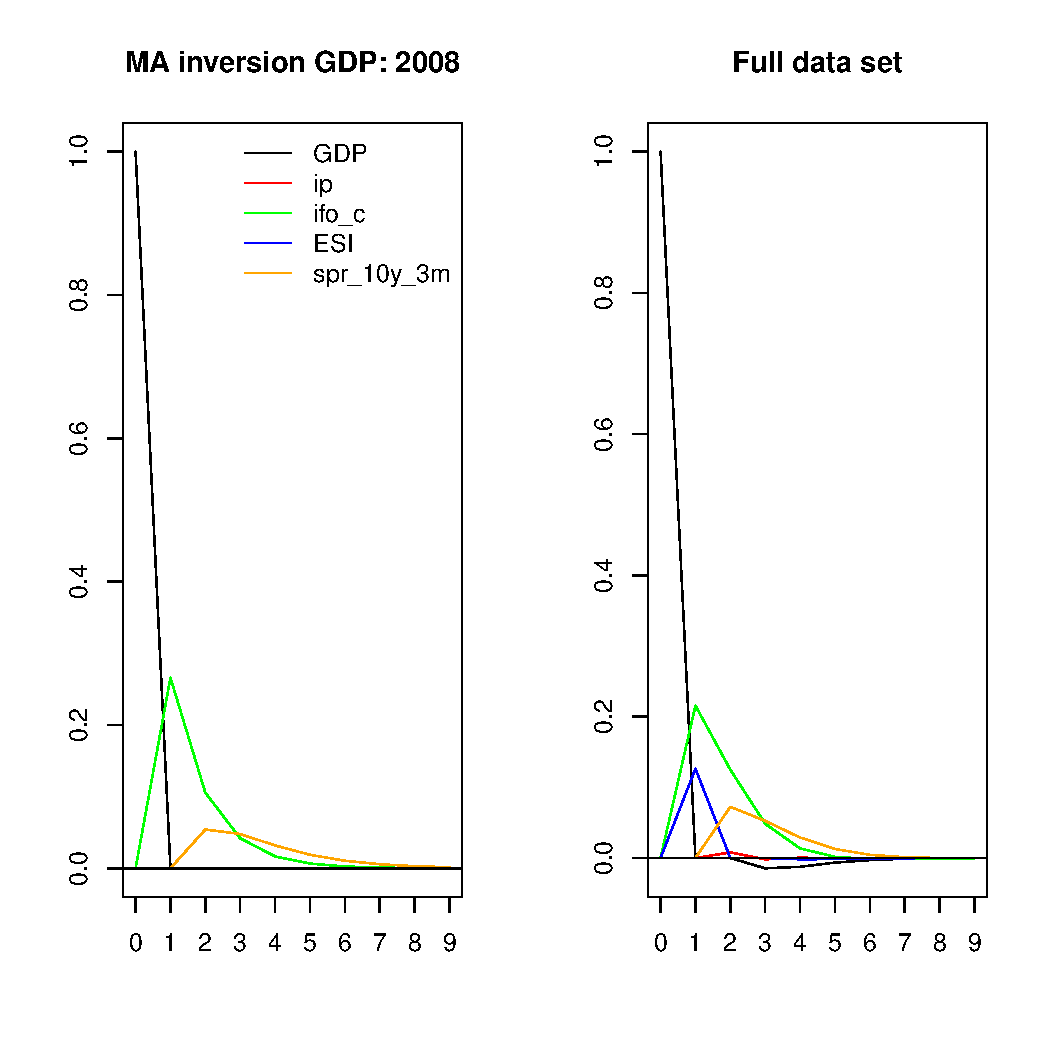
\includegraphics[height=3in, width=5in]{./Figures/up_dated_ma_inv_multi_ip.pdf}\caption{MA-inversion (impulse response) of VAR: data up to Jan-2008 (left) vs. entire data set  without pandemic (right).\label{up_dated_ma_inv_multi_ip}}\end{center}\end{figure}
\begin{figure}[H]\begin{center}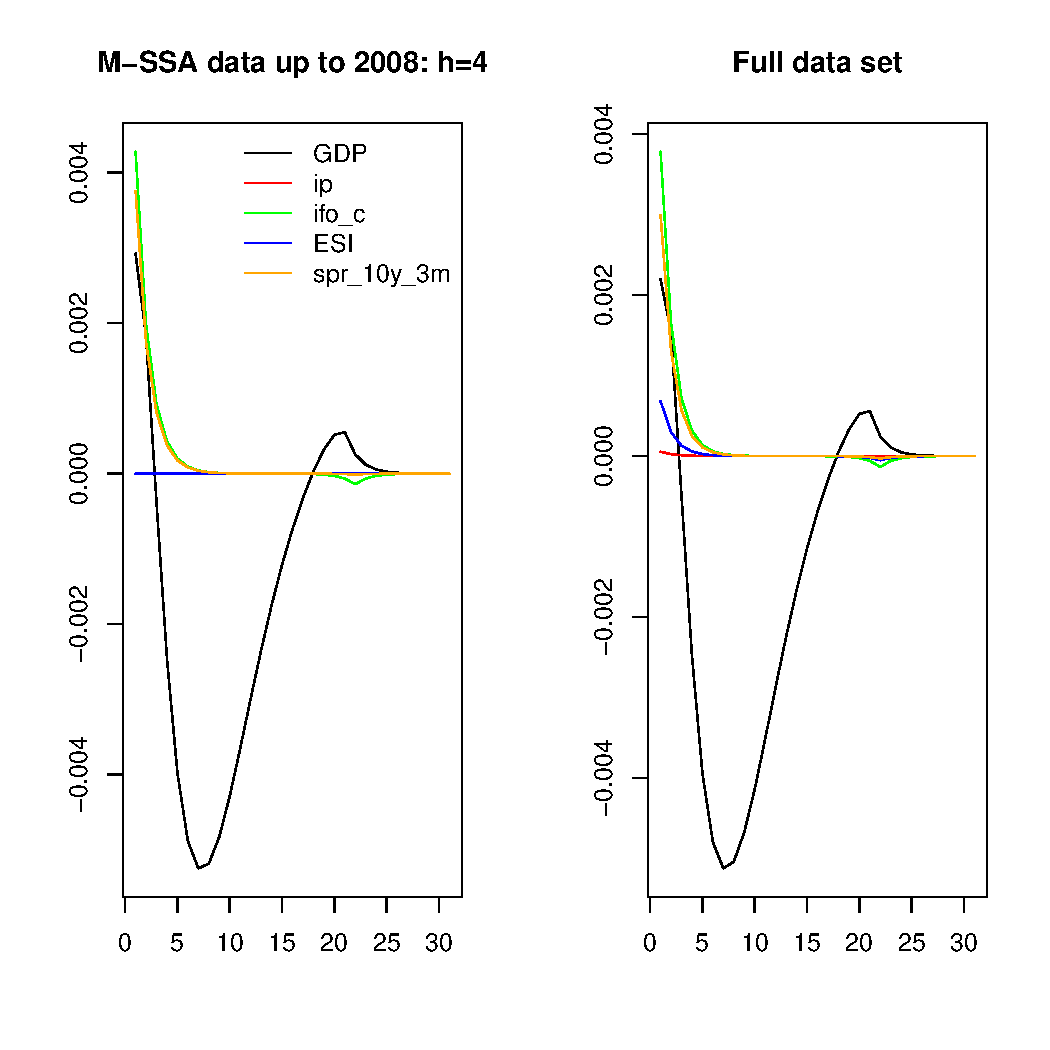
\includegraphics[height=3in, width=5in]{./Figures/bk_2008_all.pdf}\caption{M-SSA filter tracking HP-GDP at forecast horizon $h=4$: data up to Jan-2008 (left) vs. entire data set without pandemic (right).\label{bk_2008_all}}\end{center}\end{figure}

\begin{figure}[H]\begin{center}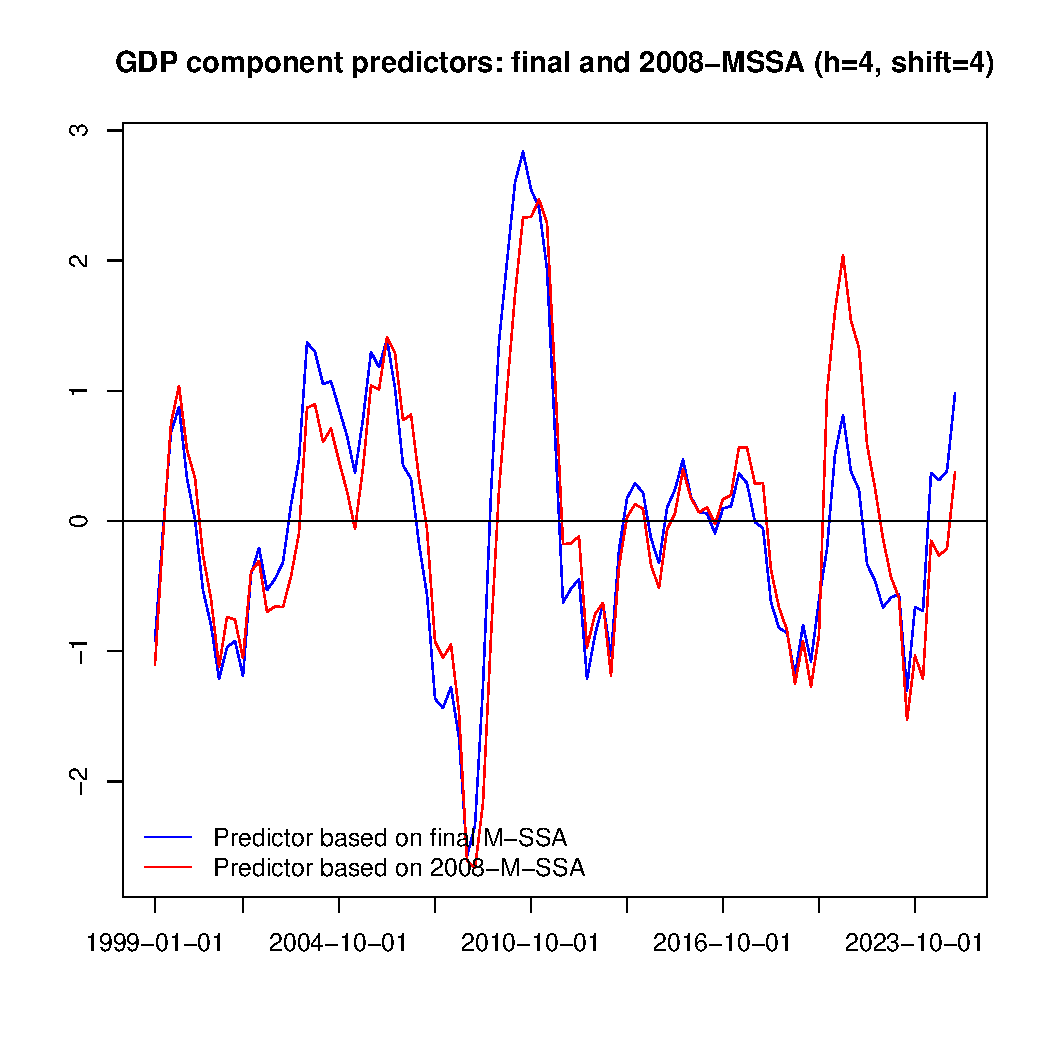
\includegraphics[height=3in, width=5in]{./Figures/revisions3.pdf}\caption{Revisions resulting from updates to the VAR model in M-SSA optimized for $h=shift=4$. To isolate the effect of the regression revision, all series are standardized. The up-dated M-SSA (blue) is left-shifted at the zero-crossings and appears slightly faster. For consistency, the entire pandemic episode has been removed.\label{revisions3}}\end{center}\end{figure}



\section{Hit Rate vs. False Alarm Rate}


%As shown in Wildi (2025), the SSA criterion's objective function—the target correlation $\rho(y,z,h)$—can be linked to the sign accuracy of the predictor $SA(y_t):=\text{P}\left(\text{sign}(z_{t+h}) = \text{sign}(y_t)\right)$, i.e., the probability that the signs of the predictor $y_t$ and the target $z_{t+h}$ agree:
%\begin{eqnarray}\label{sig_acc}
%SA(y_t)=0.5+\frac{\arcsin(\rho(y,z,h))}{\pi}.
%\end{eqnarray}
%Due to the strict monotonicity of the arcsin function, maximizing the target correlation also maximizes the sign accuracy of the predictor.\footnote{Equation \ref{sig_acc} holds exactly for Gaussian processes. Due to the central limit theorem, the relationship holds approximately for low-pass filtered non-Gaussian series, see Wildi (2025).} 
\textbf{Remarks:}
\begin{itemize}
\item Alternative to MSE, target correlation, holding-time: hit-rate, false alarm. 
\item We can link objective function (target correlation) with sign accuracy, see Wildi (2025). BUT: risk that reviewer asks for comparison with logit or whatever sign-forecast tool.
\item Context ROC-curve
\end{itemize}
For the ROC curves, we consider predictors of GDP based on both original (unfiltered) and filtered indicators. For the direct forecast, we use the regression
\[
GDP_{t+shift}=\beta_0^{shift}+\sum_{i=1}^5\beta_i^{shift}x_{ti}+\epsilon_{t}^{shift,direct}=\hat{GDP}_{t+shift}^{direct}+\epsilon_{t}^{shift,direct},
\]
where $x_{ti}$ designates the original indicators. 
For the filtered indicators, we consider similar regression equations:
\[GDP_{t+shift}=\beta_0^{shift,h,filt}+\sum_{i=1}^5\beta_i^{shift,h,filt}y_{ti}^{h,filt}+\epsilon_{t}^{h,shift,filt}=\hat{GDP}_{t+shift}^{h,filt}+\epsilon_{t}^{h,shift,filt},\]
where $y_{ti}^{h,filt}$ represents the $i$-th filtered indicator optimized at forecast horizon $h$, based on either HP-C, M-MSE, or M-SSA. \\
\textbf{Remarks:}
\begin{itemize}
\item I'm computing all combinations of shift and h. 
\item But we could emphasize the diagonal only (h=shift): simplifies notation/explanation.
\item The table of AUCs (below) is based on diagonal only
\end{itemize}
For simplicity of exposition, we present results based on the full sample, excluding the pandemic period. Fig.\ref{ROC_GDP_shift_1_4} compares ROCs of the predictors for small and mid-term forecast horizons and Table \ref{auc} presents AUCs (area under the curve) for forecast horizons 1-5 quarters ahead.




\begin{figure}[H]\begin{center}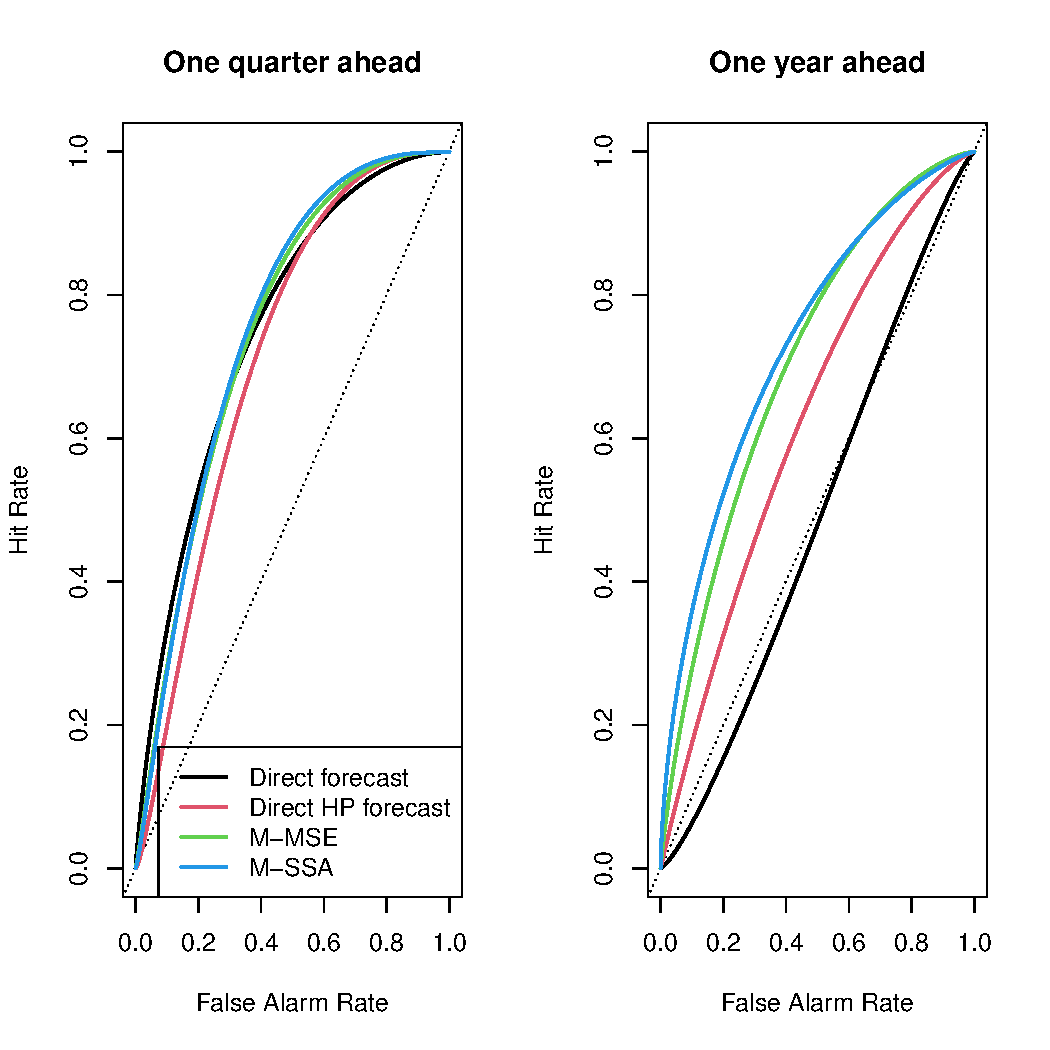
\includegraphics[height=3in, width=5in]{./Figures/ROC_GDP_shift_1_4.pdf}\caption{Hit rate vs. false alarm rate of the predictors at small (one quarter ahead:left panel) and yearly forecast horizons (right panel).\label{ROC_GDP_shift_1_4}}\end{center}\end{figure}
% latex table generated in R 4.2.2 by xtable 1.8-4 package
% Fri May 23 08:06:40 2025
\begin{table}[ht]
\centering
\begin{tabular}{rrrrr}
  \hline
 & Direct forecast & Direct HP forecast & M-MSE & M-SSA \\ 
  \hline
Forecast horizon 1 & 0.752 & 0.715 & 0.746 & 0.747 \\ 
  Forecast horizon 2 & 0.697 & 0.663 & 0.729 & 0.720 \\ 
  Forecast horizon 3 & 0.554 & 0.622 & 0.684 & 0.709 \\ 
  Forecast horizon 4 & 0.486 & 0.624 & 0.680 & 0.708 \\ 
  Forecast horizon 5 & 0.593 & 0.636 & 0.643 & 0.701 \\ 
   \hline
\end{tabular}
\caption{AUCs of predictors against GDP at various forecast horizons.} 
\label{p_val_wc5}
\end{table}At forecast horizons less than or equal to two quarters, the direct forecast challenges the filters. However, for horizons $h>2$, the filters outperform the direct approach: the univariate HP-C design is surpassed by the classic multivariate MSE filter, which is in turn dominated by the M-SSA. These results confirm that controlling the rate of sign changes of the predictor, while maximizing its target correlation through M-SSA can enhance predictor performance in terms of sign accuracy and false alarm rate.


\section{Summary and Conclusion}


Classic direct forecasts of BIP can outperform simple benchmarks, such as the mean, up to two quarters ahead. However, this limited forecast horizon is often insufficient for certain applications. A key challenge with direct forecasts is that the relevant indicators tend to be noisy, which can mask the true signal and lead to overfitting. In particular, the predictor struggles to timely track dips (slowdowns, recessions) or peaks (recoveries, expansions). To address this issue, we apply a HP(160)-filter to smooth the data, with the smoothing parameter $\lambda=160$ reflecting a more adaptive design than the classic quarterly HP, in line with an intended forecast horizon of up to one year ahead. The resulting predictor tends to outperform the classic direct forecasts in terms of statistical significance, mainly due to a slight left-shift noticeable at sharp recession dips. However, despite the filtering, the predictor remains somewhat noisy, potentially producing excessive noisy zero-crossings at the transitions between recessions and expansions. This issue is partly due to noise leakage inherent in the one-sided HP filter. \\

To address these problems, we propose a multivariate extension of SSA based on Wildi (2024). Unlike the univariate HP filter, the M-SSA can leverage cross-sectional information from indicators leading BIP in real time while controlling for the rate of zero-crossings of the predictor. Consequently, the multivariate filter outputs become increasingly left-shifted as the forecast horizon lengthens, allowing dips and peaks of the target series to be tracked more systematically, while reducing the occurrence of noisy zero-crossings. However, since M-SSA does not explicitly target BIP, an additional step is necessary to derive the final BIP predictor. We propose two approaches: a simple equally-weighted aggregate, assuming all M-SSA components are equally important for predicting BIP, and an optimally weighted predictor based on a regression of the M-SSA components on future BIP.\\

For illustration, we consider a simple approach based on regressing the single M-SSA BIP output on future BIP, thereby ignoring the other filter outputs. This predictor is intuitively appealing because the future HP-BIP—i.e., the target of M-SSA—is the low-frequency component of the future BIP target. Consequently, a strong link between M-SSA and future HP-BIP also indicates a connection with BIP, even if the statistical significance is obscured by the noise inherent in BIP. Out-of-sample performance suggests that this predictor is statistically significant at horizons up to one year. Moreover, designs optimized for larger forecast horizons outperform the mean benchmark at all considered forecast horizons, and the predictor exceeds the performance of direct forecasts—based on unfiltered or HP filtered indicators—at horizons longer than two quarters. An analysis of revision errors arising from quarterly updates of the proposed M-SSA BIP component predictor indicates that the regression parameters, the VAR model, and the resulting M-SSA filters stabilize after an initial burn-in period. This stability enhances the explainability and interpretability of the predictor.\\

In conclusion, the new predictor design integrates the traditional direct forecast approach with a novel multivariate filter to target BIP up to one year ahead. This multivariate approach leverages a set of economic indicators leading BIP in real time while controlling the smoothness of the predictor through the zero-crossing rate. 

\newpage

\section{Appendix}

\subsection{Performances: Without Pandemic}


% latex table generated in R 4.2.2 by xtable 1.8-4 package
% Fri May 23 08:06:40 2025
\begin{table}[ht]
\centering
\begin{tabular}{rrrrrrrr}
  \hline
 & h=0 & h=1 & h=2 & h=3 & h=4 & h=5 & h=6 \\ 
  \hline
Shift=0 & 0.086 & 0.049 & 0.018 & 0.005 & 0.002 & 0.002 & 0.042 \\ 
  Shift=1 & 0.238 & 0.165 & 0.097 & 0.033 & 0.005 & 0.001 & 0.005 \\ 
  Shift=2 & 0.815 & 0.680 & 0.428 & 0.180 & 0.029 & 0.007 & 0.008 \\ 
  Shift=3 & 0.866 & 0.963 & 0.922 & 0.699 & 0.269 & 0.079 & 0.047 \\ 
  Shift=4 & 0.361 & 0.808 & 0.989 & 0.954 & 0.546 & 0.127 & 0.034 \\ 
  Shift=5 & 0.351 & 0.786 & 0.982 & 0.943 & 0.579 & 0.245 & 0.042 \\ 
   \hline
\end{tabular}
\caption{HAC adjusted p-values of regressions of M-SSA component predictors optimized for forecast horizons $h=0,...,6$  (the columns) on BIP shifted forward by shift=0,...,5 (the rows). Out-of-sample span starting in Jan-2007, without pandemic.} 
\label{p_val_wc5}
\end{table}% latex table generated in R 4.2.2 by xtable 1.8-4 package
% Fri May 23 08:06:40 2025
\begin{table}[ht]
\centering
\begin{tabular}{rrrrrrrr}
  \hline
 & h=0 & h=1 & h=2 & h=3 & h=4 & h=5 & h=6 \\ 
  \hline
Shift=0 & 0.950 & 0.917 & 0.877 & 0.851 & 0.865 & 0.910 & 0.960 \\ 
  Shift=1 & 1.028 & 1.007 & 0.960 & 0.899 & 0.867 & 0.878 & 0.912 \\ 
  Shift=2 & 1.040 & 1.043 & 1.030 & 0.984 & 0.933 & 0.910 & 0.913 \\ 
  Shift=3 & 1.006 & 1.024 & 1.040 & 1.025 & 0.983 & 0.952 & 0.941 \\ 
  Shift=4 & 0.977 & 1.003 & 1.034 & 1.040 & 1.005 & 0.964 & 0.937 \\ 
  Shift=5 & 0.984 & 1.011 & 1.044 & 1.057 & 1.031 & 0.986 & 0.949 \\ 
   \hline
\end{tabular}
\caption{rRMSEs of M-SSA components predictor benchmarked against the expanding mean of BIP. Out-of-sample span starting in Jan-2007, without pandemic.} 
\label{rRMSE_mSSA_comp_mean6}
\end{table}% latex table generated in R 4.2.2 by xtable 1.8-4 package
% Fri May 23 08:06:40 2025
\begin{table}[ht]
\centering
\begin{tabular}{rrrrrrrr}
  \hline
 & h=0 & h=1 & h=2 & h=3 & h=4 & h=5 & h=6 \\ 
  \hline
Shift=0 & 1.104 & 1.066 & 1.019 & 0.989 & 1.006 & 1.058 & 1.116 \\ 
  Shift=1 & 1.232 & 1.206 & 1.150 & 1.076 & 1.038 & 1.051 & 1.092 \\ 
  Shift=2 & 1.146 & 1.150 & 1.136 & 1.085 & 1.028 & 1.002 & 1.006 \\ 
  Shift=3 & 1.008 & 1.027 & 1.042 & 1.028 & 0.986 & 0.954 & 0.943 \\ 
  Shift=4 & 0.988 & 1.014 & 1.045 & 1.051 & 1.016 & 0.975 & 0.948 \\ 
  Shift=5 & 0.967 & 0.995 & 1.027 & 1.039 & 1.013 & 0.970 & 0.933 \\ 
   \hline
\end{tabular}
\caption{rRMSEs of M-SSA components predictor benchmarked against the direct forecasts. Out-of-sample span starting in Jan-2007, without pandemic.} 
\label{rRMSE_mSSA_comp_direct_without_covid7}
\end{table}% latex table generated in R 4.2.2 by xtable 1.8-4 package
% Fri May 23 08:06:40 2025
\begin{table}[ht]
\centering
\begin{tabular}{rrrrrrr}
  \hline
 & Shift=0 & Shift=1 & Shift=2 & Shift=3 & Shift=4 & Shift=5 \\ 
  \hline
RRMSE & 0.860 & 0.835 & 0.907 & 0.998 & 0.989 & 1.017 \\ 
   \hline
\end{tabular}
\caption{rRMSEs direct forecasts benchmarked against the expanding mean. Out-of-sample span starting in Jan-2007, without pandemic.} 
\label{rRMSE_mSSA_direct_mean_without_covid8}
\end{table}

\newpage
\subsection{Performances: Including Singular Pandemic Data}

% latex table generated in R 4.2.2 by xtable 1.8-4 package
% Fri May 23 08:06:40 2025
\begin{table}[ht]
\centering
\begin{tabular}{rrrrrrrr}
  \hline
 & h=0 & h=1 & h=2 & h=3 & h=4 & h=5 & h=6 \\ 
  \hline
Shift=0 & 0.142 & 0.074 & 0.023 & 0.003 & 0.001 & 0.002 & 0.013 \\ 
  Shift=1 & 0.475 & 0.344 & 0.217 & 0.111 & 0.044 & 0.023 & 0.044 \\ 
  Shift=2 & 0.724 & 0.564 & 0.325 & 0.101 & 0.023 & 0.010 & 0.012 \\ 
  Shift=3 & 0.943 & 0.979 & 0.933 & 0.670 & 0.234 & 0.066 & 0.031 \\ 
  Shift=4 & 0.322 & 0.666 & 0.960 & 0.946 & 0.644 & 0.263 & 0.119 \\ 
  Shift=5 & 0.386 & 0.721 & 0.940 & 0.910 & 0.591 & 0.248 & 0.060 \\ 
   \hline
\end{tabular}
\caption{HAC adjusted p-values of regressions of M-SSA component predictors optimized for forecast horizons $h=0,...,6$  (the columns) on BIP shifted forward by shift=0,...,5 (the rows). Out-of-sample span starting in Jan-2007, including the pandemic.} 
\label{p_val1}
\end{table}% latex table generated in R 4.2.2 by xtable 1.8-4 package
% Fri May 23 08:06:40 2025
\begin{table}[ht]
\centering
\begin{tabular}{rrrrrrrr}
  \hline
 & h=0 & h=1 & h=2 & h=3 & h=4 & h=5 & h=6 \\ 
  \hline
Shift=0 & 0.991 & 0.974 & 0.952 & 0.933 & 0.929 & 0.942 & 0.965 \\ 
  Shift=1 & 1.037 & 1.030 & 1.012 & 0.985 & 0.966 & 0.963 & 0.969 \\ 
  Shift=2 & 1.014 & 1.014 & 1.005 & 0.983 & 0.959 & 0.950 & 0.953 \\ 
  Shift=3 & 1.010 & 1.017 & 1.021 & 1.011 & 0.988 & 0.969 & 0.961 \\ 
  Shift=4 & 0.987 & 0.999 & 1.015 & 1.020 & 1.008 & 0.992 & 0.981 \\ 
  Shift=5 & 0.996 & 1.008 & 1.023 & 1.030 & 1.018 & 0.997 & 0.976 \\ 
   \hline
\end{tabular}
\caption{rRMSEs of M-SSA components predictor benchmarked against the expanding mean of BIP. Out-of-sample span starting in Jan-2007, including the pandemic.} 
\label{rRMSE_mSSA_comp_mean2}
\end{table}% latex table generated in R 4.2.2 by xtable 1.8-4 package
% Fri May 23 08:06:40 2025
\begin{table}[ht]
\centering
\begin{tabular}{rrrrrrrr}
  \hline
 & h=0 & h=1 & h=2 & h=3 & h=4 & h=5 & h=6 \\ 
  \hline
Shift=0 & 1.228 & 1.207 & 1.180 & 1.156 & 1.151 & 1.167 & 1.196 \\ 
  Shift=1 & 0.978 & 0.972 & 0.955 & 0.929 & 0.912 & 0.908 & 0.915 \\ 
  Shift=2 & 1.030 & 1.029 & 1.021 & 0.998 & 0.974 & 0.964 & 0.968 \\ 
  Shift=3 & 1.037 & 1.044 & 1.048 & 1.038 & 1.014 & 0.995 & 0.986 \\ 
  Shift=4 & 0.973 & 0.985 & 1.000 & 1.006 & 0.994 & 0.978 & 0.966 \\ 
  Shift=5 & 0.981 & 0.993 & 1.008 & 1.015 & 1.003 & 0.982 & 0.962 \\ 
   \hline
\end{tabular}
\caption{rRMSEs of M-SSA components predictor benchmarked against the direct forecasts. Out-of-sample span starting in Jan-2007, including the pandemic.} 
\label{rRMSE_mSSA_comp_direct3}
\end{table}% latex table generated in R 4.2.2 by xtable 1.8-4 package
% Fri May 23 08:06:40 2025
\begin{table}[ht]
\centering
\begin{tabular}{rrrrrrr}
  \hline
 & Shift=0 & Shift=1 & Shift=2 & Shift=3 & Shift=4 & Shift=5 \\ 
  \hline
RRMSE & 0.807 & 1.060 & 0.985 & 0.974 & 1.015 & 1.015 \\ 
   \hline
\end{tabular}
\caption{rRMSEs direct forecasts benchmarked against the expanding mean. Out-of-sample span starting in Jan-2007, including the pandemic.} 
\label{rRMSE_mSSA_direct_mean4}
\end{table}





\end{document}
